%% TopoGuard: Adaptive Topology Orchestration for Risk-Sensitive Decision
%% under Hard Constraints and Multimodal Uncertainty
%% Submitted to ACM Transactions on Multimedia Computing, Communications and Applications (TOMM)
%%
%% Commands for TeXCount
%TC:macro \cite [option:text,text]
%TC:macro \citep [option:text,text]
%TC:macro \citet [option:text,text]
%TC:envir table 0 1
%TC:envir table* 0 1
%TC:envir tabular [ignore] word
%TC:envir displaymath 0 word
%TC:envir math 0 word
%TC:envir comment 0 0
%%
\documentclass[acmsmall,review,anonymous]{acmart}

\usepackage{graphicx}
\usepackage{amsmath,amsfonts}
\usepackage{booktabs}
\usepackage{algorithm}
\usepackage{algpseudocode}
\setlength{\headheight}{20.5pt}
\addtolength{\topmargin}{-7.5pt}

\setcopyright{none}
\settopmatter{printacmref=true}
\renewcommand\footnotetextcopyrightpermission[1]{}


%%
%% \BibTeX command to typeset BibTeX logo in the docs
\AtBeginDocument{%
  \providecommand\BibTeX{{%
    Bib\TeX}}}


%%
%% end of the preamble, start of the body of the document source.
\begin{document}

%%
%% The "title" command has an optional parameter,
%% allowing the author to define a "short title" to be used in page headers.
\title{TopoGuard: Adaptive Topology Orchestration for Risk-Sensitive Decision Systems under Hard Constraints and Multimodal Uncertainty}



%%
%% The abstract is a short summary of the work to be presented in the
%% article.
\begin{abstract}
Risk-sensitive decision-support systems, such as storm-surge warning and emergency response, increasingly rely on multi-stage collaboration among heterogeneous modules and multimodal evidence, including textual requests, sensor time-series, and spatial forecast products. Such systems face a dual challenge: multimodal uncertainty, such as noisy sensors or conflicting weather patterns, can destabilize evidence reliability, while hard operational constraints, such as safety thresholds, strict time windows, and mandatory human oversight, make unconstrained trial-and-error or full online replanning difficult to justify. Fixed pipelines are easy to deploy but brittle across structurally diverse task instances. We propose \textbf{TopoGuard}, a profile-guided framework for workflow-structure-level adaptation in multimodal decision support. Instead of exhaustive online search, TopoGuard maintains task-conditional quality--cost--latency profiles for candidate workflow topologies (auditable DAG prototypes) and executor assignments, uses constrained Pareto selection to choose an initial topology aligned with the current task difficulty and operational constraints, and records execution feedback for future profile update. Evaluator modules can monitor intermediate output quality and trigger bounded local repair when failures occur; the repair procedure upgrades only affected stages rather than replanning the entire workflow. Using a trace-based evaluation with frozen profiles over held-out execution records from a water-conservancy digital-twin platform, TopoGuard nearly matches the quality-maximizing baseline ($S=0.902$ vs.\ $0.914$) while reducing latency (77.6\,s vs.\ 118.9\,s), and outperforms fixed pipelines, executor-only routing, and offline-search proxy baselines. These results suggest that auditable topology orchestration can serve as a practical structure-level adaptation mechanism for multimodal decision support, achieving near quality-maximizing performance with lower latency and bounded recovery under operational constraints.
\end{abstract}

%%
%% The code below is generated by the tool at http://dl.acm.org/ccs.cfm.
%% Please copy and paste the code instead of the example below.
%%
\begin{CCSXML}
<ccs2012>
   <concept>
       <concept_id>10002951.10003227.10003241</concept_id>
       <concept_desc>Information systems~Decision support systems</concept_desc>
       <concept_significance>500</concept_significance>
   </concept>
   <concept>
       <concept_id>10002951.10003227.10003251</concept_id>
       <concept_desc>Information systems~Multimedia information systems</concept_desc>
       <concept_significance>500</concept_significance>
   </concept>
   <concept>
       <concept_id>10010147.10010178</concept_id>
       <concept_desc>Computing methodologies~Artificial intelligence</concept_desc>
       <concept_significance>300</concept_significance>
   </concept>
   <concept>
       <concept_id>10010147.10010178.10010199</concept_id>
       <concept_desc>Computing methodologies~Planning and scheduling</concept_desc>
       <concept_significance>300</concept_significance>
   </concept>
</ccs2012>
\end{CCSXML}

\ccsdesc[500]{Information systems~Decision support systems}
\ccsdesc[500]{Information systems~Multimedia information systems}
\ccsdesc[300]{Computing methodologies~Artificial intelligence}
\ccsdesc[300]{Computing methodologies~Planning and scheduling}

%%
%% Keywords. The author(s) should pick words that accurately describe
%% the work being presented. Separate the keywords with commas.
\keywords{Multimedia Systems, Topology Orchestration, Multimodal Decision Support, Workflow Adaptation, Local Graph Repair, Digital Twin}
%% A "teaser" image appears between the author and affiliation
%% information and the body of the document, and typically spans the
%% page.

\begin{teaserfigure}
\centering
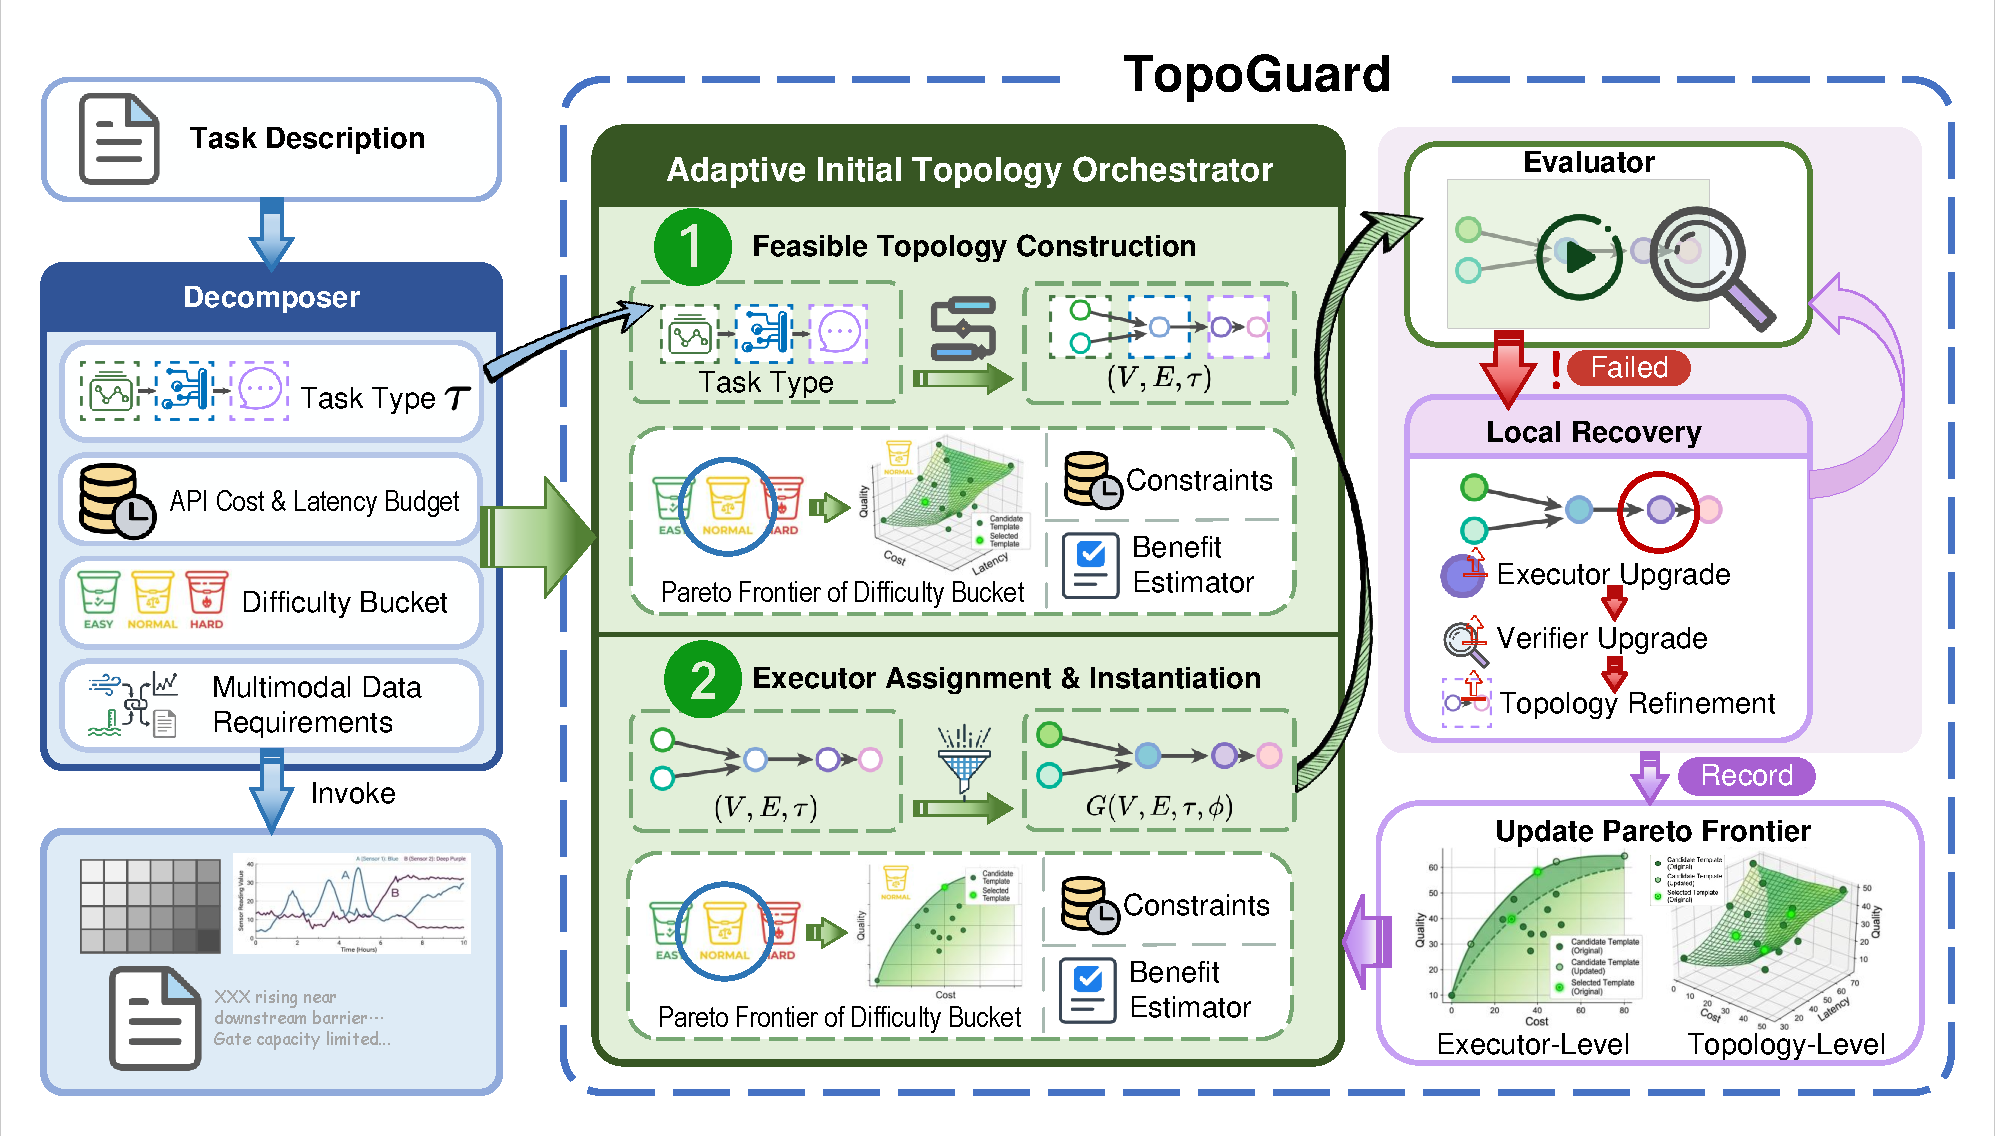
\includegraphics[width=\linewidth]{figures/fig2_v2.pdf}
\caption{Overview of TopoGuard. Given a task description, resource constraints, and heterogeneous multimodal evidence, TopoGuard selects an auditable workflow prototype, assigns executors, monitors intermediate outputs, and applies bounded local recovery when failures occur.}
\Description{Workflow diagram showing task inputs, resource constraints, and multimodal evidence entering TopoGuard; the system consults learned profiles, selects an auditable DAG prototype, assigns executors, monitors intermediate quality, and applies local repair before producing decision-support outputs.}
\label{fig:framework}
\end{teaserfigure}

% \received{20 February 2007}
% \received[revised]{12 March 2009}
% \received[accepted]{5 June 2009}

%%
%% This command processes the author and affiliation and title
%% information and builds the first part of the formatted document.
\maketitle

\section{Introduction}
Modern multimodal intelligent systems are increasingly used for decision support in risk-sensitive domains such as hydrological analysis, infrastructure monitoring, and emergency response \cite{algiriyage2022multi,cheng2023review,inyang2025digital,tomczak2024development,yuan2024digitaltwin,zhang2023multimodalfusion}. In these settings, task completion typically requires the coordinated use of heterogeneous functional modules, including data retrieval, numerical computation, reasoning, and verification \cite{zhang2024mm,huang2024understanding,zhai2025survey}. System effectiveness therefore depends not only on individual executors, but also on how they are organized into an executable collaboration topology.

However, such systems face a dual challenge: multimodal uncertainty (e.g., noisy sensors or conflicting weather patterns) destabilizes evidence reliability, while hard constraints (e.g., safety thresholds, strict time windows, and mandatory human oversight) prohibit unconstrained online exploration. Many deployed systems still rely on manually designed workflows or fixed model-selection rules where functional nodes and execution order are predetermined \cite{zeng2023flowmind,li2024autoflow,zhang2024aflow,fan2024workflowllm}. Such designs are easy to deploy but brittle in uncertain environments: different task instances require different processing structures; intermediate outputs may fail; and execution must satisfy constraints on quality, cost, and latency. A workflow that performs well for one instance may become expensive, slow, or ineffective for another, especially in risk-sensitive applications where local failures can propagate into unreliable downstream decisions \cite{tang2016emergency}. This issue is further amplified in multimodal settings with missing or unreliable modalities \cite{wu2024mlmmsurvey,lan2025robust,reza2024robust,liaqat2025chameleon,zhang2023multimodalfusion,zhou2023foundation}. In these settings, trial-and-error exploration is often infeasible because failed executions may consume scarce response time or violate operational safeguards.

Existing approaches attempt to improve adaptability through tool use, reasoning-action loops, and parallel function scheduling \cite{schick2023toolformer,yao2023react,kim2024llm}. However, the core decision is not only which executor to use, but also which functional nodes should be activated, how they should be connected, and how the execution graph should be adjusted when failures occur. In other words, the decision variable is the workflow topology itself. Recent work on LLM planning, graph execution, and workflow generation highlights structured execution organization, but mainly focuses on planning quality rather than topology adaptation under execution-time constraints \cite{huang2024understanding,zhai2025survey,li2024autoflow,zhang2024aflow,fan2024workflowllm,huang2023dag,peled2021graph}. We therefore formulate the problem as \emph{adaptive topology orchestration} under hard constraints and multimodal uncertainty, focusing on how multimedia evidence streams are routed, verified, and selectively invoked rather than on learning a new cross-modal representation.

To address this problem, we propose \textbf{TopoGuard}, an adaptive topology orchestration framework for risk-sensitive multimodal decision support. TopoGuard treats workflow execution as a closed-loop decision process over structured graphs. It maintains task-conditional quality--cost--latency profiles for candidate auditable workflow DAG prototypes and executor assignments. Based on these profiles, TopoGuard performs constrained Pareto-based selection to obtain an initial executable graph aligned with the current task difficulty and operational constraints. During execution, evaluator modules monitor intermediate outputs and detect local failures or reliability risks. Instead of triggering global replanning, TopoGuard performs bounded local graph repair that upgrades only affected stages while preserving reusable upstream computation.

A central observation motivating this work is that multimodal decision-support systems can benefit from choosing and maintaining appropriate \emph{collaboration topologies}, rather than relying only on component selection within a fixed pipeline. Topology-level adaptation allows the execution graph to adjust to task requirements, resource constraints, and execution-time uncertainty, which is relevant for balancing effectiveness, efficiency, and reliability in risk-sensitive environments.

We evaluate TopoGuard on representative tasks involving heterogeneous executors and structured workflow operators. Experimental results show that TopoGuard nearly matches the quality-maximizing baseline while reducing latency, outperforming fixed workflows, executor-only routing, and single-objective baselines. Additional analyses indicate that bounded local repair provides useful recovery when intermediate execution quality degrades, and that topology-level adaptation is especially relevant when task instances differ in structural requirements.

\noindent\textbf{The main contributions of this paper are summarized as follows:}
\begin{itemize}
    \item \textbf{Problem Formulation.} We formulate adaptive workflow execution in risk-sensitive multimodal decision support as adaptive topology orchestration over auditable workflow prototypes under hard resource constraints and heterogeneous multimodal evidence.
    \item \textbf{TopoGuard Framework.} We propose \textbf{TopoGuard}, a feasibility-aware topology orchestration framework that integrates offline performance profiling, constrained Pareto-based initial topology selection, and evaluator-triggered bounded local repair.
    \item \textbf{Empirical Validation.} We evaluate TopoGuard using a trace-based protocol with frozen profiles over recorded digital-twin execution traces and show that it nearly matches the quality-maximizing baseline while reducing latency, outperforming fixed pipelines, executor-only routing, and offline-search proxy baselines. Component analyses further indicate that topology selection and executor adaptation are the main average-performance drivers, while local repair provides targeted recovery after detected intermediate failures.
\end{itemize}

\section{Related Work}
\label{sec:related_work}

\subsection{Multimedia Decision Support and Digital Twins in High-Stakes Domains}

Multimedia systems are increasingly used beyond perception and retrieval, and have become part of decision-support pipelines in high-stakes settings such as emergency response, infrastructure monitoring, and hydrological analysis \cite{tang2016emergency,pathak2020hydroinformatics,yu2024warenet}. In water and infrastructure domains, recent digital-twin studies emphasize real-time monitoring, simulation, and decision support as core capabilities of intelligent management systems \cite{li2024intelligentwater,ge2025urbanflooddt}. These systems typically integrate heterogeneous observations, simulation outputs, and operational knowledge, but their execution logic is often implemented as manually designed pipelines or domain-specific control flows. Our work is related to this line of research in that it also targets decision support under multimodal inputs and operational constraints. The difference is that we focus on \emph{how} the execution structure should be selected and adjusted during execution when task requirements, resource limits, and intermediate reliability vary across instances.

\subsection{Multimodal Uncertainty and Missing-Modality Robustness}

A large body of multimodal research studies robustness under missing, noisy, or unreliable inputs \cite{lan2025robust,wu2024mlmmsurvey}. This literature is directly relevant because real-world decision systems often operate with partial observability, degraded sensors, or cross-source inconsistency. Existing methods mainly improve robustness within a fixed model architecture or a fixed processing pipeline, for example through missing-modality learning, representation completion, or robust fusion. By contrast, we examine a different question: when evidence quality changes, should the system still use the same execution structure, or should it switch to a different workflow topology with additional verification or recovery stages? In this sense, our work complements model-level robustness methods by addressing structure-level adaptation.

\subsection{Workflow and Agent Orchestration}

Recent work on LLM-based agents has highlighted the value of structured execution rather than single-shot prompting. ReAct and Tree of Thoughts illustrate how intermediate reasoning and tool interaction can improve complex task solving \cite{yao2023react,yao2023tot}. More recent workflow-oriented approaches explicitly treat agent execution as a graph or workflow construction problem. For example, AFlow formulates agentic workflow generation as search over code-represented workflows and optimizes node-edge structure automatically \cite{zhang2024aflow}. These studies show that execution structure matters, but they primarily focus on producing strong workflows or better reasoning performance. Our setting is different in two respects: we consider hard deployment constraints on cost and latency during selection, and we explicitly model bounded local repair after execution has started.

\subsection{Cost-Aware Routing, Cascading, and Runtime Recovery}

Another closely related line of research studies cost-aware model selection and cascading. FrugalGPT shows that routing or cascading across models can reduce inference cost while maintaining strong task performance \cite{chen2023frugalgpt}. Subsequent work further unifies routing and cascading and highlights the importance of quality estimation for cost-performance trade-offs \cite{dekoninck2024routing,gao2024constraintaware,liu2024risk}. These methods are relevant because they also optimize quality under budget constraints, but they usually treat the decision variable as \emph{which model} to call for a given query. Our work instead treats the workflow topology itself as the decision variable, jointly considering node activation, graph structure, executor assignment, and local repair.

Our repair component is also related to the broader literature on workflow exception handling and adaptive failure recovery. Prior research in workflow systems and service composition has studied exception handling, ad-hoc recovery, online recovery, and adaptive failure handling for composite processes \cite{chiu2001exception,sato2010adaff,hutter2023online,wang2023adaptive}. Those studies motivate the importance of execution-time recovery, but they are generally not formulated around modern multimodal agent workflows or multi-objective quality-cost-latency trade-offs. We build on the same general intuition that failures should be handled locally when possible, while instantiating it in a profile-guided orchestration framework for multimodal decision systems.









\section{Method}
\label{sec:method}

\subsection{Problem Setup}

We consider adaptive orchestration for multi-stage decision tasks. For an input task $X$, the system must choose (i) a workflow structure, (ii) executor assignments for the nodes in that structure, and (iii) a limited set of repair actions if execution quality falls below a threshold.

The framework has two coupled stages: initial topology selection under hard cost--latency constraints and quality-oriented utility, followed by bounded local repair when intermediate failures are detected. Because the workflow-graph space is combinatorial, direct search is impractical; we therefore use a hierarchical selection procedure together with minimal-change local repair.

\medskip
\noindent\textbf{Multimodal Input and Output Specification.}
The system operates on heterogeneous multimodal inputs and produces multi-format outputs. Concretely, the input to a task instance comprises:

\begin{itemize}
    \item \textbf{Sensor time-series data}: hydrological measurements (water level, flow rate, temperature) sampled at regular intervals.
    \item \textbf{Forecast products}: heterogeneous meteorological outputs including spatial fields (wind velocity, precipitation maps), scalar indices (storm surge height, wave period), and probabilistic forecast envelopes.
    \item \textbf{Textual queries}: natural-language task descriptions, user questions, or domain-specific instructions.
\end{itemize}

These multimodal inputs are passed through workflow nodes that may consume different modality combinations. For example, a retrieval node processes textual queries against a knowledge base; a computation node takes sensor time-series and produces scalar or vector diagnostics; a reasoning node consumes both textual context and numerical outputs from upstream computation. The workflow output similarly spans multiple modalities: temporal evolution curves, spatial comparison maps, statistical summaries, and natural-language warnings or explanations. This heterogeneous input--output structure is characteristic of the multimedia decision-support setting and motivates the need for topology-level adaptation: different modality combinations may call for different processing structures depending on which modalities are available, noisy, or conflicting during execution.

\subsection{Initial Topology Selection under Hard Constraints}
\label{sec:init_objective}

We first formulate the construction of the initial executable workflow as a constrained topology selection problem, following the general multi-objective view that operational decisions should be evaluated jointly over utility, resource use, and feasibility \cite{gonzalez2022constrained,miettinen2010nonlinear,sun2023pareto,tian2024constraint}.
Given an input task $X$, the policy $\pi$ selects an initial workflow graph $G_{\pi}(X)$ from the candidate graph space.
The objective is to maximize utility under hard structural and resource constraints:
\begin{equation}
\pi^\star
=
\arg\max_{\pi\in\Pi}
\;\mathbb{E}_{X\sim D}\big[Q(G_{\pi}(X),X)\big],
\label{eq:init_obj}
\end{equation}
subject to
\begin{equation}
\begin{aligned}
&G_{\pi}(X)\in\mathcal{G}_{\mathrm{DAG}},\\
&C(G_{\pi}(X),X)\le B(X),\\
&L(G_{\pi}(X),X)\le \Delta(X).
\end{aligned}
\label{eq:init_constraints}
\end{equation}

Here, $\mathcal{G}_{\mathrm{DAG}}$ denotes the space of valid directed acyclic workflow graphs,
$B(X)$ is the task-specific budget constraint, and $\Delta(X)$ is the latency constraint.
This stage determines only the \emph{initial} executable topology; repair actions during execution are formulated separately in Section~\ref{sec:repair}.

To compare quality, cost, and latency on a comparable scale, we use a normalized utility:
\begin{equation}
Q(G,X)=\alpha\,S_{\mathrm{norm}}(G,X)-\beta\,C_{\mathrm{norm}}(G,X)-\gamma\,L_{\mathrm{norm}}(G,X),
\label{eq:utility}
\end{equation}
where $\alpha,\beta,\gamma\ge 0$ and $\alpha+\beta+\gamma=1$.
In our implementation, quality is normalized as
\begin{equation}
S_{\mathrm{norm}}(G,X)=\frac{S(G,X)}{S_{\mathrm{scale}}},
\label{eq:s_norm}
\end{equation}
and cost and latency use the normalized profile values $C_{\mathrm{norm}}$ and $L_{\mathrm{norm}}$ for candidate comparison.
Unless otherwise specified, we use $\alpha=0.65$, $\beta=0.25$, $\gamma=0.10$, and $S_{\mathrm{scale}}=1.5$.
Pareto frontiers are used only for candidate pruning before the final utility-based selection.

\subsection{Workflow Representation}

A workflow is represented as a directed graph
\begin{equation}
G=(V,E,\tau,\rho,\phi),
\end{equation}
where $V$ is the node set, $E\subseteq V\times V$ is the directed edge set, $\tau(v)$ is node role type, $\rho(v)$ is executor function type, and $\phi(v)$ is runtime configuration. DAG topology is enforced by a topological order $\operatorname{ord}:V\rightarrow\{1,\dots,|V|\}$ such that
\begin{equation}
(u,v)\in E\Rightarrow \operatorname{ord}(u)<\operatorname{ord}(v).
\end{equation}

Task context is encoded into a discrete difficulty level $b \in \{\text{easy}, \text{medium}, \text{hard}\}$, estimated from task features such as query length, domain complexity, and retrieval scope. The resulting difficulty level is used to condition both template retrieval and executor candidate selection.

In the current implementation, topology adaptation is instantiated as selection over a controlled space of auditable workflow DAG prototypes rather than unrestricted DAG generation. Each prototype is defined over typed functional nodes, including retrieval, reasoning, computation, verification, and aggregation, and corresponds to a valid executable topology with profiled quality--cost--latency behavior. The four prototypes used in our experiments (direct, fallback-direct, executor--verifier, and executor--verifier--aggregator) are representative structures in this controlled topology space. This design is intentional for risk-sensitive deployments, where candidate structures must be inspectable, profileable, and safe to execute. Our claim is therefore template-guided adaptive topology orchestration over auditable DAG prototypes, not arbitrary topology learning from scratch; larger template libraries, including parallel or hierarchical structures, can be incorporated once sufficient profile data are available. The framework itself is agnostic to the size of the template library: the same selection procedure applies whether the candidate pool contains 4 prototypes or 40.

\subsection{Profile Learning}

TopoGuard uses historical execution traces to estimate two coupled kinds of profiles. A \emph{topology-prototype profile} summarizes the expected quality, cost, and latency of a candidate DAG prototype under a task context, while an \emph{executor profile} summarizes the same quantities for assigning a concrete executor to a typed workflow node. Thus, the profile is not attached only to an executor or only to a topology node; it is indexed by the tuple
\[
(\text{node type},\text{difficulty},\text{topology prototype},\text{executor}).
\]
For each tuple observed in the training split, we aggregate execution records to obtain
\[
\widehat{S}=\mathrm{mean}(S),\qquad
\widehat{C}=\mathrm{mean}(C),\qquad
\widehat{L}=\mathrm{mean}(L),
\]
together with empirical standard deviations and sample counts. Cost and latency are additionally log-normalized for Pareto filtering and utility ranking, while raw values are retained for reporting. Topology-level selection marginalizes over the profiled candidates belonging to the same prototype and context; node-level selection then chooses the executor assignment within the selected prototype. During evaluation, these profiles are frozen: all strategies choose from profile estimates, and held-out realized quality, cost, and latency are used only after a candidate has been selected. Execution feedback is logged as future profile data but is not used to update the profile within the same test batch.

\subsection{Difficulty-Aware Hierarchical Initialization}

Given task $X$ and difficulty level $b$, initialization is decomposed into two levels:
\begin{equation}
T_0=\pi_{\text{init}}^{T}(X,b),
\qquad
\Phi_0=\pi_{\text{init}}^{N}(X,b,T_0),
\qquad
G_0=(T_0,\Phi_0).
\end{equation}

At the topology-prototype level, we first perform Pareto pruning over candidate workflow DAG prototypes:
\begin{equation}
\mathcal{P}_T=\text{Pareto}_{\max S,\min C,\min L}(\mathcal{T}(X,b)),
\end{equation}
and then select the feasible topology prototype with highest proxy utility:
\begin{equation}
T_0=\arg\max_{T\in\mathcal{P}_T^{\text{feasible}}}\widehat{Q}_T(T;X,b).
\end{equation}

At the node level, each executor node retrieves a difficulty-conditioned candidate pool,
\begin{equation}
\mathcal{A}_v(b,\rho(v)),
\qquad
\mathcal{P}_N(v)=\text{Pareto}_{\max S,\min C}(\mathcal{A}_v(b,\rho(v))),
\end{equation}
and selects the feasible candidate with maximal utility:
\begin{equation}
Q_N(a;v,X,b)=\alpha_N S(a;v,X,b)-\beta_N C(a;v,X,b),
\end{equation}
\begin{equation}
\phi(v)=\arg\max_{a\in\mathcal{P}_N^{\text{feasible}}(v)}Q_N(a;v,X,b).
\end{equation}

\subsection{Bounded Local Repair with Edit-Loss}
\label{sec:repair}

After the initial workflow $G_0$ has been selected and instantiated, execution proceeds in a closed loop.
When the evaluator detects that an intermediate result fails the pass condition, TopoGuard does not re-optimize the whole graph from scratch.
Instead, it performs bounded local repair around the affected region.
This repair module is an integral execution-time adaptation layer of TopoGuard: initial topology orchestration chooses the starting workflow, while bounded repair maintains that workflow when local execution quality degrades.

At execution step $t$, let $G_t$ denote the current workflow graph and $s_t$ the local execution state.
A repair action is selected as
\begin{equation}
a_t=\pi_{\mathrm{repair}}(s_t),
\qquad
G_{t+1}=\mathcal{T}_{\mathrm{op}}(G_t,a_t),
\label{eq:repair_transition}
\end{equation}
where $\mathcal{T}_{\mathrm{op}}$ applies a local graph edit to the current workflow.

We consider four concrete bounded repair routes,
\begin{equation}
\mathcal{A}_t=\{A,B,C_1,C_2\},
\end{equation}
where $A$ denotes topology/template upgrade, $B$ denotes executor upgrade within the current topology, $C_1$ denotes cross-topology executor upgrade, and $C_2$ denotes verifier/evaluator upgrade.
To discourage unnecessary large edits, we define the edit loss as
\begin{equation}
\mathcal{L}_{\mathrm{edit}}(a)
=
\lambda_n\Delta n(a)+\lambda_\phi\Delta\phi(a)+\lambda_e\Delta e(a),
\label{eq:edit_loss}
\end{equation}
where $\Delta n(a)$, $\Delta\phi(a)$, and $\Delta e(a)$ measure changes in nodes, executor assignments, and edges.
In our implementation, the weights are set to $\lambda_n=0.30$, $\lambda_\phi=0.25$, $\lambda_e=0.10$, and the overall penalty weight is $\lambda=0.20$.

The repair policy then solves a bounded local optimization problem:
\begin{equation}
a_t^\star
=
\arg\max_{a\in\mathcal{A}_t^{\mathrm{feasible}}}
\Big(
Q(G_{t+1}(a),X)-\lambda\,\mathcal{L}_{\mathrm{edit}}(a)
\Big),
\label{eq:repair_obj}
\end{equation}
where the feasible repair set is
\begin{equation}
\mathcal{A}_t^{\mathrm{feasible}}
=
\{a\in\mathcal{A}_t \mid S(G_{t+1}(a),X)\ge\tau_{\mathrm{pass}}\}.
\label{eq:repair_feasible}
\end{equation}
Here $\tau_{\mathrm{pass}}=0.5432$ is the data-driven repair trigger threshold (the 25th percentile of quality scores across training-profile entries in the Water QA benchmark), which is computed once from training data and held fixed at evaluation time. During repair selection, $S$ and $Q$ are profile-based estimates; held-out realized quality is used only after the repaired workflow has been selected.

This formulation separates repair from initial topology selection:
the initial stage chooses a globally feasible workflow under hard constraints, whereas repair performs \emph{local correction} aimed at restoring execution quality without global replanning.

\begin{algorithm}[t]
\caption{TopoGuard Hierarchical Pareto Orchestration}
\label{alg:hpo}
\begin{algorithmic}[1]
\Require Task $X$, performance profile $\mathcal{P}$, budget $B$, latency bound $\Delta$, repair threshold $\tau_{\mathrm{pass}}$
\Ensure Final workflow $G^*$ and execution result
\State $b \gets \textsc{EstimateDifficulty}(X)$ \Comment{estimate task difficulty level}
\State $\mathcal{F}_T \gets \textsc{ParetoFilter}(\mathcal{P}, b, B, \Delta)$ \Comment{topology-prototype-level Pareto pruning}
\State $T_0 \gets \arg\max_{T \in \mathcal{F}_T} \hat{Q}(T; X, b)$ \Comment{select highest-utility topology prototype}
\For{each $v \in V(T_0)$}
    \State $\mathcal{F}_v \gets \textsc{ParetoFilter}(\mathcal{P}, v, b, B)$ \Comment{node-level Pareto pruning}
    \State $\phi(v) \gets \arg\max_{a \in \mathcal{F}_v} Q_N(a; v, X, b)$ \Comment{select best executor}
\EndFor
\State Execute workflow $G_0 = (T_0, \Phi_0)$, obtain intermediate outputs $\{o_v\}$
\For{each $v \in V(T_0)$}
    \If{$\textsc{Evaluator}(o_v) < \tau_{\mathrm{pass}}$} \Comment{evaluator detects local failure}
        \State $\mathcal{A}_{\mathrm{feas}} \leftarrow
\{a \in \{A,B,C_1,C_2\} \mid \widehat{S}(G(a),X) \ge \tau_{\mathrm{pass}}\}$
        \State $a^\star \leftarrow
\arg\max_{a\in\mathcal{A}_{\mathrm{feas}}}
\left[\widehat{Q}(G(a),X)-\lambda\mathcal{L}_{\mathrm{edit}}(a)\right]$
        \State $G_0 \leftarrow \mathcal{T}_{\mathrm{op}}(G_0,a^\star)$ \Comment{apply bounded local repair}
    \EndIf
\EndFor
\State Log execution feedback for future profile updates; \Return $G^* \gets G_0$
\end{algorithmic}
\end{algorithm}


\section{Experiments}
\label{sec:experiments}

We evaluate TopoGuard using a trace-based protocol with frozen profiles over held-out execution records collected from a water-conservancy digital-twin platform. 
For each task instance, the system first selects an executable workflow under quality--cost--latency constraints and then monitors execution for possible local repair. 
The experiments are organized around the following questions:

\begin{itemize}
    \item \textbf{RQ1:} Can TopoGuard achieve a strong quality--cost--latency trade-off relative to the baselines?
    \item \textbf{RQ2:} Do topology-prototype selection and executor adaptation provide complementary gains over fixed, routing-only, and offline-searched workflows?
    \item \textbf{RQ3:} Do the observed advantages remain stable across task domains and different utility preferences?
    \item \textbf{RQ4:} When intermediate execution quality degrades, can bounded local repair provide targeted recovery without global replanning?
\end{itemize}

\subsection{Experimental Setup}
\label{subsec:exp_setup}



\paragraph{Platform and task domains.}
We conduct all experiments on a water-conservancy digital-twin platform and evaluate TopoGuard on two representative task domains: \textbf{Water QA} and \textbf{Storm Surge}. 
The primary benchmark, \textbf{Water QA}, is formulated as a multi-stage question answering task over hydrological knowledge. 
Different task instances may require different execution structures, such as retrieval, reasoning, computation, verification, and aggregation. 
Multimodal uncertainty is reflected in both the evidence interface and the task difficulty dimension: easy, medium, and hard instances differ in query ambiguity, retrieval noise, and the reliability of intermediate outputs, while storm-surge tasks additionally involve heterogeneous forecast artifacts such as temporal curves, spatial maps, scalar metrics, and textual warning requirements. The benchmark is therefore designed around structure-level multimodal decision support: it evaluates whether the workflow topology should adapt when different modality combinations and reliability levels are required. The auxiliary benchmark, \textbf{Storm Surge}, is used to examine whether the same orchestration rule can be applied to another decision domain without redesigning the core decision logic.


\paragraph{Data and evaluation protocol.}
For Water QA, we construct a benchmark containing training and test executions, which are further aggregated into historical performance profiles for candidate workflows and executors. 
For Storm Surge, we build an auxiliary transfer benchmark with heterogeneous execution choices and evaluate whether the same orchestration strategy can be applied to a second task domain without redesigning the decision rule. 
In both domains, the training split is used to estimate the expected quality, cost, and latency of candidate workflows, while all final results are reported on held-out execution records. Profiles are frozen during evaluation; execution feedback is logged for future updates but is not used to update profiles within the same test batch.
The reported $S$, cost, and latency are therefore realized held-out outcomes after a candidate workflow has been selected, not the profile estimates used for selection.
Thus, the main Water QA and Storm Surge results are trace-based recorded-execution evaluations with frozen profiles over platform executions, not purely synthetic simulations; only the stress and perturbation diagnostics inject controlled test-time degradations.

Given a test context, the system first queries historical profiles to estimate the expected triplet $(S,C,L)$ for each candidate topology or executor, applies hard constraint filtering, computes the feasible Pareto frontier, and then selects an execution plan according to the corresponding orchestration strategy.
For TopoGuard, the selected plan is further executed in a closed loop with evaluator monitoring and optional local repair.
The repair trigger uses intermediate realized quality signals during execution; it does not observe the final held-out quality before deciding whether to repair.

Table~\ref{tab:benchmark_stats} summarizes the benchmark construction statistics. The Water QA benchmark comprises 17 models $\times$ 5 node types $\times$ 3 difficulty levels, yielding 163 non-empty profile entries. Some rare combinations lack feasible candidates after hard cost--latency filtering; under the default constraints, 221 of 255 held-out contexts have at least one feasible candidate and are included in the main feasible-set comparison. The global Pareto frontier contains 48 non-dominated feasible profile candidates. All profiles are estimated from training records on the same platform; no external data is used.

\begin{table}[t]
\centering
\caption{Benchmark construction statistics for the Water QA domain.}
\label{tab:benchmark_stats}
\small
\begin{tabular}{lr}
\toprule
\textbf{Item} & \textbf{Count / Value} \\
\midrule
Candidate models & 17 \\
Node types & 5 (retrieval, reasoning, computation, verification, aggregation) \\
Difficulty levels & 3 (easy, medium, hard) \\
Topology templates & 4 (direct, fallback-direct, executor+verifier, executor+verifier+aggregator) \\
Profile entries & 163 \\
Pareto frontier size & 48 \\
Training records & 1,467 \\
Test contexts (unique) & 255 (221 feasible under default constraints) \\
Test episodes (total) & 834 \\
Constraint budget $C_{\max}$ & 0.5 (log-normalized) \\
Latency budget $L_{\max}$ & 0.90 (log-normalized) \\
$Q$-score scale $S_{\text{scale}}$ & 1.5 \\
\bottomrule
\end{tabular}
\end{table}

The multimodal nature of the benchmark is reflected in both input and output artifacts: textual queries, hydrological time-series, spatial forecast fields, scalar measurements, and heterogeneous outputs including curves, maps, summaries, and warning text. Different workflow nodes consume different modality combinations, which is why topology selection rather than executor routing alone is central to the evaluation.

\paragraph{Compared methods.}
We compare seven orchestration methods, including TopoGuard and six baselines, organized by whether they select from the Pareto feasible candidate pool:

\textbf{Candidate-pool selection methods} (selecting from the profile-derived feasible candidate pool; the Water QA global Pareto frontier contains 48 non-dominated candidates):
\begin{itemize}
    \item \textbf{TopoGuard (dual-layer adaptive):} performs Pareto pruning and utility-maximization selection at both the template level and the executor level, with bounded local repair. This is the full framework proposed in this paper.
    \item \textbf{LLM Router (executor-only adaptive):} selects the best executor by estimated quality within a fixed topology template (executor+verifier), without adapting workflow structure. Models the common model-routing approach and isolates the contribution of topology-level adaptation.
    \item \textbf{AFlow-Style (offline-searched):} searches for a globally optimal (topology, executor) combination on the training split using the same utility function, then fixes this workflow for all test contexts without task-conditional adaptation. This baseline is inspired by offline workflow-search methods such as AFlow and AutoFlow, but is instantiated within our controlled auditable topology space and does not constitute a full reproduction of \cite{zhang2024aflow}, which targets unconstrained code-generation and planning workflows. It therefore serves as a proxy baseline for fixed offline workflow search rather than a direct reproduction.
    \item \textbf{Best-Quality / Profile-Cheapest:} select the candidate with the highest estimated quality or the lowest estimated cost, respectively. Because reported cost is realized execution cost, FrugalGPT Cascade can occasionally have lower realized cost than Profile-Cheapest.
\end{itemize}

\textbf{Fixed-pipeline methods} (not selecting from the candidate pool):
\begin{itemize}
    \item \textbf{Static Workflow:} fixes the topology to executor+verifier and the executor to Kimi-K2.5. No Pareto screening, no adaptive topology selection, and no repair. This conservative non-adaptive pipeline serves as an alternative operating point for evaluating the quality-overhead trade-off.
    \item \textbf{FrugalGPT Cascade:} sorts executors by cost and selects the first meeting $S \geq 0.70$, without topology adaptation. Models the ``call cheap model first, escalate only if needed'' strategy.
\end{itemize}

This organization highlights the core innovation of TopoGuard---dual-layer adaptive topology selection---and provides controlled comparisons that isolate the contribution of each adaptive layer. The AFlow-Style comparison tests whether task-conditional adaptation provides value beyond offline workflow search, while the Static Workflow comparison evaluates whether the adaptive overhead is worthwhile in practice.


\paragraph{Metrics.}
We report three primary metrics: \textbf{quality} $S\in[0,1]$, \textbf{cost} $C$ (USD), and \textbf{latency} $L$ (seconds).
Quality measures the final task-solving effectiveness of the selected workflow.
Cost is computed from actual execution expenses, and latency records the realized end-to-end execution delay.
Following the current implementation, cost and latency are log-normalized only for internal Pareto filtering, while all reported results use raw values for interpretability.

The quality score $S$ is computed with the same evaluator protocol for all compared methods. For each executed node or final workflow output, the evaluator applies the task-appropriate rubric and normalizes the resulting score to $[0,1]$. Objective sub-tasks use direct task metrics when available; open-ended decision-support outputs use judge-proxy rubrics covering correctness, completeness, constraint satisfaction, and clarity. Workflow-level $S$ is the realized held-out quality attached to the selected execution record, whereas profile-level $\widehat{S}$ is estimated only from training records and used for selection. Thus, the reported $S$ values are not observed by any strategy before choosing a candidate.

We do not report violation rate as a discriminative metric in the main comparison because feasibility filtering is applied before selection; however, feasible coverage is reported because some contexts have no candidate under the hard filters. Note on constraint scope: our experiments apply a single global cost budget $C_{\max}=0.5$ and latency budget $L_{\max}=0.9$ (log-normalized) uniformly across all 255 test contexts, rather than per-context constraints. This corresponds to a deployed platform setting where all tasks share the same operational resource ceiling. The constraint stress test (Section~\ref{subsec:sensitivity}) varies $C_{\max}$ around the default value to evaluate robustness to moderate budget changes.


The internal selection metric $Q(G;X)=\alpha S_{\text{norm}}-\beta C_{\text{norm}}-\gamma L_{\text{norm}}$ is used solely for Pareto frontier ranking and candidate tie-breaking; it does not appear as a reported evaluation metric. $S_{\text{norm}}=S / S_{\text{scale}}$ normalizes quality to the same scale as $C_{\text{norm}}$ and $L_{\text{norm}}$, preventing quality from dominating the score purely due to scale differences. In our implementation, $(\alpha,\beta,\gamma)=(0.65,0.25,0.10)$ with $S_{\text{scale}}=1.5$, which balances quality prioritization with genuine cost-latency trade-offs on the Pareto frontier.

\subparagraph{Experiment protocol.}\label{subsubsec:exp_protocol}
Our experiments consist of two complementary evaluation protocols:
\textbf{(1) Shared-pool controlled comparison}: Best-Quality and Profile-Cheapest are evaluated as controlled selection baselines on the same learned profiles, selecting from the shared feasible candidate pool. This isolates the effect of the decision heuristic while holding the candidate space fixed.
\textbf{(2) Operating-point comparison}: TopoGuard and Static Workflow are evaluated on the same test contexts but represent different deployment philosophies (adaptive vs.\ fixed). They are not compared on a single metric; instead, the two are contrasted on their respective strengths: TopoGuard on quality and adaptive robustness, Static Workflow on cost-efficiency and simplicity.

\paragraph{Implementation details.}
The full TopoGuard pipeline consists of: 
(1) initial context analysis, 
(2) workflow-level candidate screening, 
(3) node-level executor selection, 
(4) execution and evaluator monitoring, and 
(5) bounded local repair. 
The repair operators are defined as four bounded routes: topology/template upgrade (operator A), executor upgrade within the current topology (operator B), cross-topology executor upgrade (operator C1), and verifier/evaluator upgrade (operator C2). In the training-profile recorded-execution replay diagnostic, 231 of 585 node-level execution events trigger repair monitoring (39.5\%); this diagnostic is reported separately from the main held-out strategy comparison in Section~\ref{subsec:ablation_repair}.

\subsection{Main Results on Water QA}
\label{subsec:main_results}

\begin{figure}[t]
    \centering
    
\includegraphics[width=0.96\textwidth]{figures/fig2_overall_comparison.png}
\caption{Overall Water QA comparison. TopoGuard nearly matches the quality-maximizing profile-based baseline while improving over fixed, cascade, routing-only, and offline-search proxy baselines.}
    \Description{Four-panel comparison of Water QA strategies: quality, cost, latency, and quality-cost trade-off. TopoGuard is close to Best-Quality in quality while occupying a lower-latency operating point than the quality-maximizing baseline.}
    \label{fig:strategy_comparison_2x2}
\end{figure}

We first examine \textbf{RQ1}, namely whether TopoGuard achieves a strong quality--cost--latency trade-off on the Water QA benchmark.

Table~\ref{tab:water_qa_main} reports the trace-based evaluation results with frozen profiles on the feasible held-out Water QA contexts. The benchmark contains 255 held-out contexts and 834 held-out execution records; 221 contexts have at least one candidate after hard cost--latency feasibility filtering and are included in the main comparison.

Figure~\ref{fig:strategy_comparison_2x2} visualizes the same trend as Table~\ref{tab:water_qa_main}: TopoGuard stays close to Best-Quality in quality while avoiding the highest-cost operating point. 

\textbf{TopoGuard (adaptive)} reaches $S=0.902$ through profile-guided topology and executor selection. Best-Quality achieves a marginally higher quality ($S=0.914$), but with higher latency ($118.9$\,s vs.\ $77.6$\,s) and similar cost ($6.47\times10^{-3}$ vs.\ $6.40\times10^{-3}$ USD). Thus, TopoGuard should be interpreted as a balanced operating point rather than a single-metric optimum. On paired per-context comparison against Static Workflow ($n=221$, 204 wins / 0 ties / 17 losses), TopoGuard leads with a mean advantage of $\Delta S=+0.176$ ($0.902$ vs.\ $0.726$).

\textbf{Cost-adjusted paired regression.} To examine whether the quality gain is merely caused by higher resource use, we fit a paired regression between quality improvement and cost increase across the 221 feasible paired contexts: $\beta_0=+0.1266$ (intercept), $\beta_1=+8.8038$ (marginal return), with Cohen's $d=1.0704$ (large effect). The positive intercept suggests that TopoGuard's advantage cannot be explained solely by additional cost; the quality improvement includes a component unrelated to resource investment. We treat this analysis as supportive rather than causal evidence, and use the component ablation in Section~\ref{subsec:ablation_repair} to more directly isolate the roles of executor adaptation and topology-prototype selection.

\textbf{Static Workflow (fixed)} represents a conservative baseline with the executor+verifier topology and Kimi-K2.5 executor, without adaptive selection. The choice of executor+verifier (2-node) rather than executor+verifier+aggregator (3-node) reflects typical Water QA task requirements, where aggregation is not always necessary. It achieves lower quality ($S=0.726$) but also lower cost ($C=8.03\times10^{-4}$ USD) and latency ($L=43.5$\,s). The comparison therefore should not be read as TopoGuard dominating every operating point; rather, TopoGuard moves the feasible operating point toward substantially higher quality under the same profile-filtered candidate library.

\begin{table}[t]
\centering
\caption{Equal-budget fixed-topology comparison. Win rate and $\Delta S$ are computed over contexts where the fixed topology has a candidate under TopoGuard's per-context selection cost ceiling.}
\label{tab:strong_static}
\small
\begin{tabular}{lccc}
\toprule
\textbf{Fixed topology} & \textbf{TopoGuard win rate} & \textbf{$\Delta S$} & \textbf{Cost ratio} \\
\midrule
direct & 93.4\% & $+0.110$ & matched \\
executor+verifier & 65.0\% & $+0.044$ & matched \\
executor+verifier+aggregator & 0.0\% & $-0.030$ & matched \\
\bottomrule
\end{tabular}
\end{table}

\textbf{FrugalGPT Cascade} and \textbf{LLM Router} represent established baselines from the literature. FrugalGPT Cascade ($S=0.757$, $C=0.953\times10^{-3}$ USD, $L=67.9$\,s) escalates greedily through executors ordered by cost until a quality threshold is met, without any topology adaptation. LLM Router ($S=0.856$, $C=6.56\times10^{-3}$ USD, $L=76.4$\,s) selects the best executor within a fixed topology template, adapting only the model choice. The gap between LLM Router and TopoGuard ($\Delta S \approx +0.046$) isolates the contribution of topology-level adaptation (see Section~\ref{subsec:ablation_repair}).

\begin{figure*}[t]
    \centering
    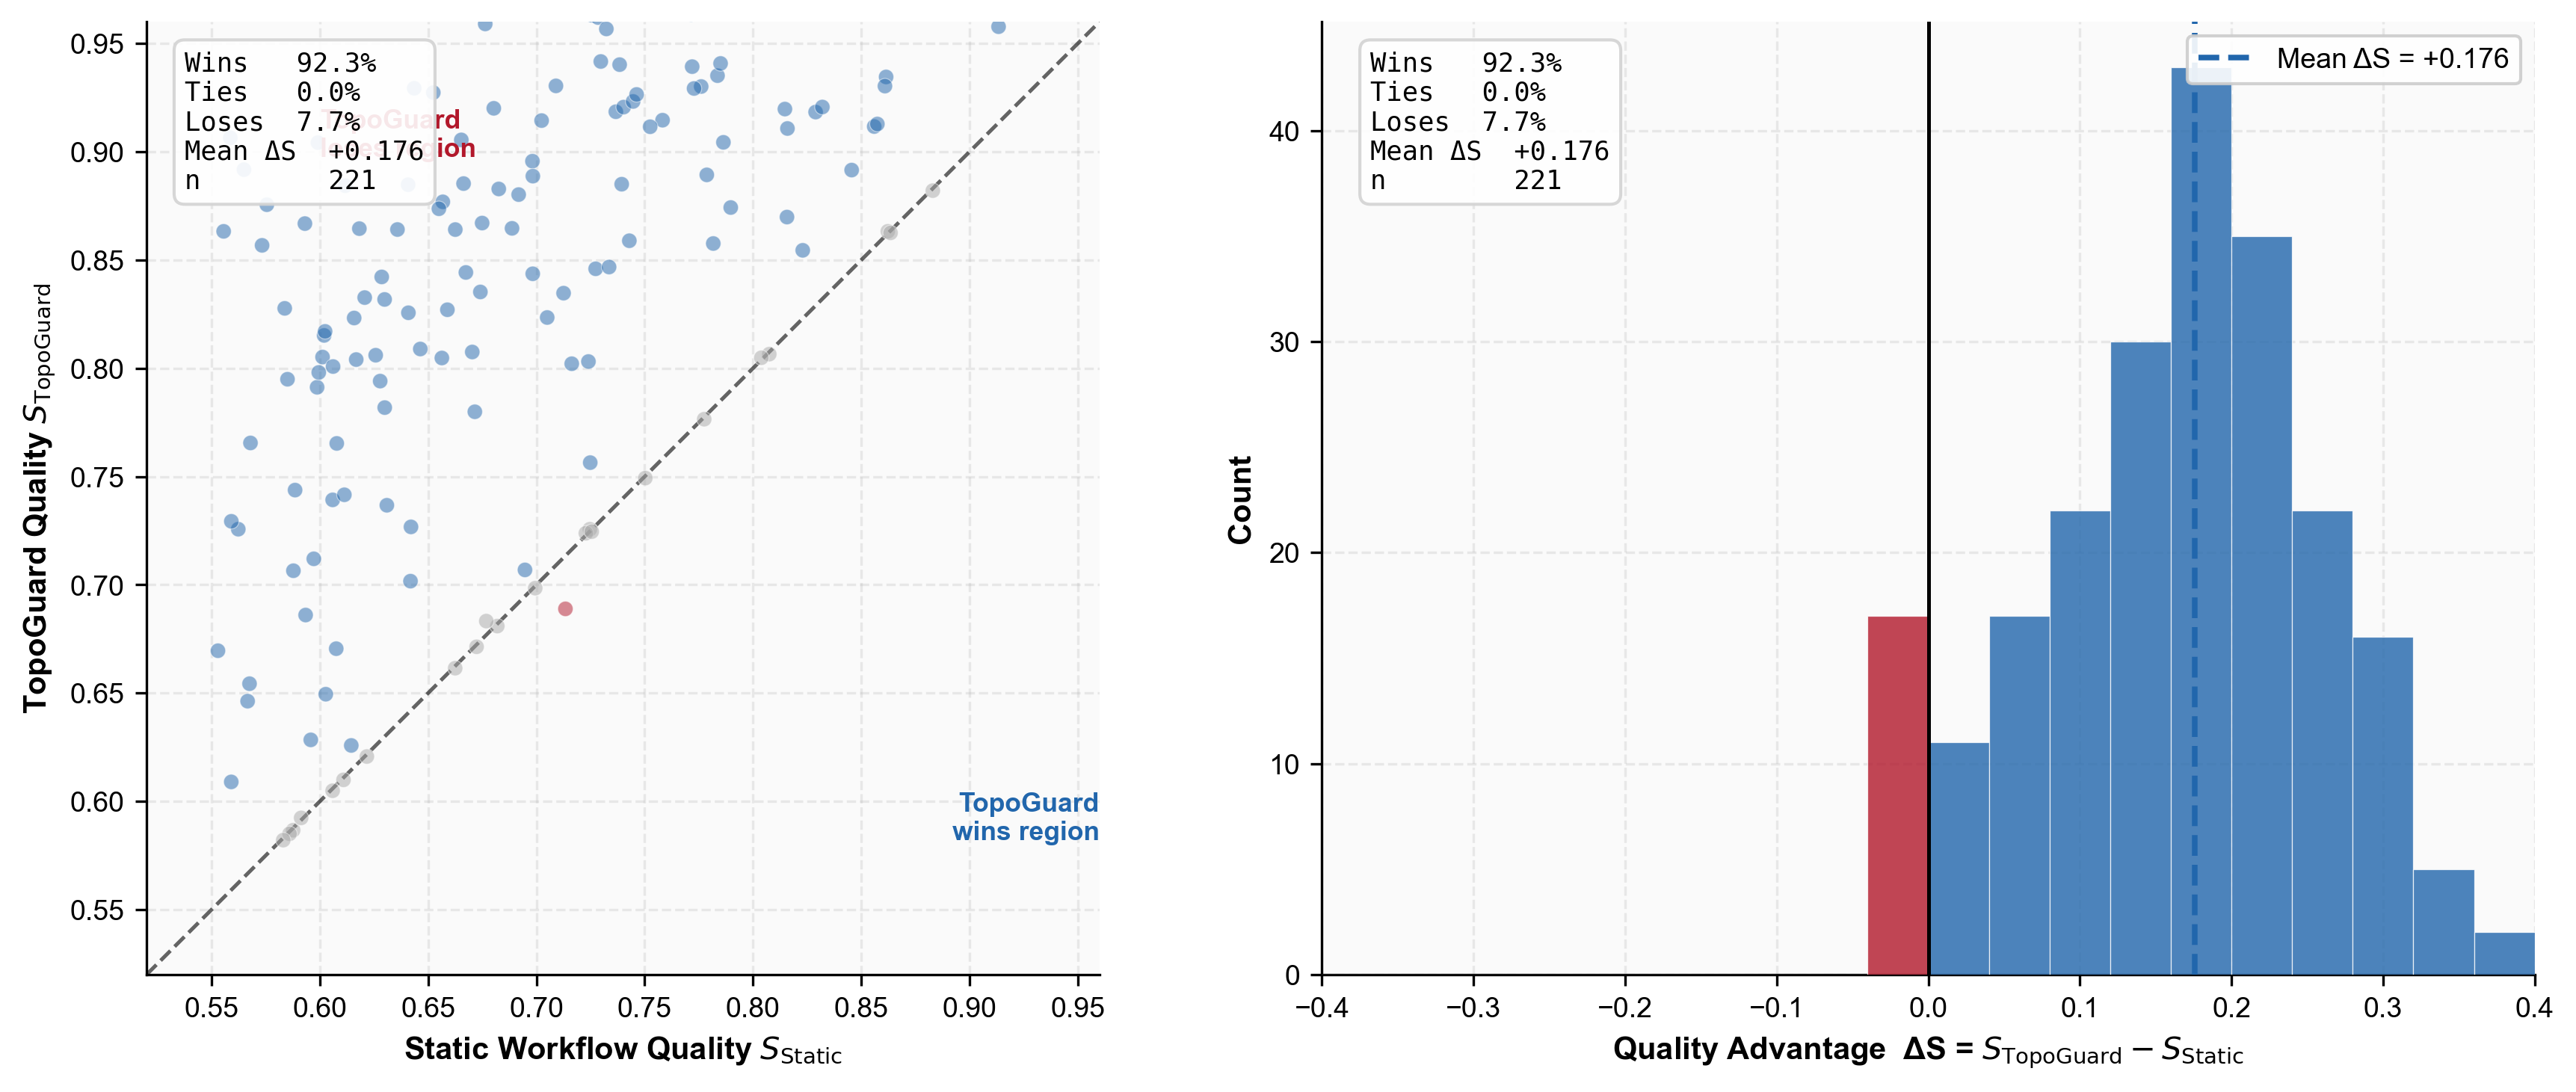
\includegraphics[width=0.96\textwidth]{figures/fig3_paired_comparison.png}
    \Description{Left: per-context scatter plot of TopoGuard quality vs Static Workflow quality. Right: histogram of per-context quality advantage delta S.}
    \caption{Per-context comparison of TopoGuard and Static Workflow. TopoGuard wins in 204/221 paired feasible contexts (92.3\%) with a mean quality advantage of $\Delta S=+0.176$.}
    \label{fig:paired_scatter}
\end{figure*}

Additional Pareto-frontier visualizations of the feasible quality--cost and quality--latency spaces are provided in the Online Appendix.

\begin{table}[t]
\centering
\caption{Closed-loop topology orchestration results on Water QA. All methods are evaluated on the same feasible held-out contexts after cost--latency filtering. Candidate-pool methods use the same profile-derived feasible pool. Best-Quality selects the candidate with the highest estimated quality $S$ from this pool and represents the quality-maximizing operating point achievable through profile-based selection without a utility trade-off. AFlow-Style is a fixed offline-search proxy, not a full reproduction of \cite{zhang2024aflow}.}
\label{tab:water_qa_main}
\resizebox{0.98\linewidth}{!}{
\begin{tabular}{lcccc}
\toprule
\textbf{Method} & \textbf{Quality $S$ $\uparrow$} & \textbf{Cost ($\times 10^{-3}$ USD) $\downarrow$} & \textbf{Latency (s) $\downarrow$} & \textbf{N} \\
\midrule
TopoGuard                                     & 0.902          & 6.40      & 77.6 & 221 \\
AFlow-Style Offline Search~\cite{zhang2024aflow} & 0.851      & 4.38      & 54.3  & 221 \\
LLM Router~\cite{kim2024llm}                  & 0.856          & 6.56      & 76.4  & 221 \\
Static Workflow                               & 0.726          & 0.80      & \textbf{43.5} & 221 \\
FrugalGPT Cascade~\cite{chen2023frugalgpt}    & 0.757          & 0.95 & 67.9 & 221 \\
Best-Quality                                  & \textbf{0.914} & 6.47      & 118.9 & 221 \\
Profile-Cheapest                              & 0.706          & \textbf{0.73}      & 56.3  & 194 \\
\bottomrule
\end{tabular}}
\end{table}

\textbf{TopoGuard quality by difficulty.} Table~\ref{tab:difficulty_breakdown} reports TopoGuard's quality at each difficulty level. TopoGuard's absolute quality decreases from easy ($S=0.920$) and medium ($S=0.915$) to hard ($S=0.851$), consistent with harder instances having noisier profiles and lower base quality. Static Workflow and LLM Router do not adapt topology selection conditioned on difficulty, so their overall scores ($S=0.726$ and $S=0.856$, respectively) are reported without per-difficulty breakdowns. The overall gains over Static Workflow and LLM Router are reported in Table~\ref{tab:water_qa_main}; Table~\ref{tab:difficulty_breakdown} is intended only to diagnose TopoGuard's own difficulty sensitivity.

\textbf{Difficulty-sensitivity analysis.} TopoGuard remains strong across all difficulty levels, but its absolute score is lower on hard contexts ($S=0.851$, $n=51$) than on easy and medium contexts ($n=85$ each). This pattern indicates that profile-guided selection remains useful under harder instances, while still leaving room for more accurate profile estimation and richer repair actions in the highest-uncertainty cases.

\begin{table}[t]
\centering
\caption{TopoGuard quality by difficulty level on Water QA. Baseline values are overall averages over the same feasible-context evaluation and should not be interpreted as per-difficulty comparisons.}
\label{tab:difficulty_breakdown}
\small
\begin{tabular}{lccc}
\toprule
\textbf{Method} & \textbf{Easy} & \textbf{Medium} & \textbf{Hard} \\
\midrule
TopoGuard        & \textbf{0.920} & \textbf{0.915} & \textbf{0.851} \\
Static Workflow (overall) & \multicolumn{3}{c}{0.726} \\
LLM Router (overall)       & \multicolumn{3}{c}{0.856} \\
\bottomrule
\end{tabular}
\end{table}



\subsection{Per-Context and Pareto Analysis}
\label{subsec:pareto_analysis}

To further interpret the trade-off, we examine per-context quality differences between TopoGuard and the main reference baselines.

Figure~\ref{fig:paired_scatter} shows the paired comparison between TopoGuard and Static Workflow at the context level. Points above the diagonal correspond to contexts in which TopoGuard achieves higher quality. The win rate is 204/221 (92.3\%, 0 ties, 17 losses), with a mean advantage of $\Delta S = +0.176$. Ties require both methods to select identical (topology, executor) pairs with identical realized quality; because TopoGuard's executor assignment always differs from Static Workflow's fixed Kimi-K2.5, zero ties occur. Relative to Best-Quality, the paired comparison shows 0 wins / 136 ties / 85 losses (mean $\Delta S = -0.012$), indicating that TopoGuard trades a small quality loss for substantially lower latency.



\subsection{Auxiliary Transfer Evidence: Storm Surge}
\label{subsec:transfer}

We also report auxiliary cross-task evidence by applying the same orchestration logic, utility weights, and selection procedure to the Storm Surge benchmark. Domain-specific profiles are estimated from Storm Surge training traces, but the orchestration rule and hyperparameters are not redesigned.
To obtain statistically meaningful comparisons, we augment the 30 held-out test tasks with up to six noise-perturbed variants and then apply the same feasibility filtering as in Water QA; therefore, the effective number of valid contexts differs across strategies ($N=144$--$168$).

Table~\ref{tab:storm_transfer} shows that TopoGuard reaches $S=0.886$ in the auxiliary transfer setting, higher than Static Workflow ($S=0.818$, $\Delta S=+0.068$), and Profile-Cheapest ($S=0.842$, $\Delta S=+0.047$). Best-Quality achieves $S=0.896$ but at 24\% higher cost ($C=2.95\times10^{-2}$ USD vs $2.38\times10^{-2}$); TopoGuard stays closer to Best-Quality in quality while using 24\% lower cost and 16\% lower latency ($S=0.886$ vs $0.896$).
An additional point of interest is the topology preference shown in Figure~\ref{fig:topo_heatmap}: TopoGuard selects a mixture of direct, executor+verifier, and executor+verifier+aggregator prototypes on Water QA (7.7\%, 23.1\%, and 69.2\%, respectively), while shifting further toward executor+verifier+aggregator on Storm Surge (88.1\%). Static Workflow remains fixed at executor+verifier in both domains. The selection distributions show that TopoGuard changes its topology choice across domains, whereas Static Workflow keeps the same executor+verifier structure.

Because the Storm Surge result uses noise-perturbed repeats from a smaller held-out set, the transfer result should be read as auxiliary evidence. The consistent topology adaptation and the advantage over the fixed-pipeline baseline are the main takeaways.

\begin{figure*}[t]
    \centering
    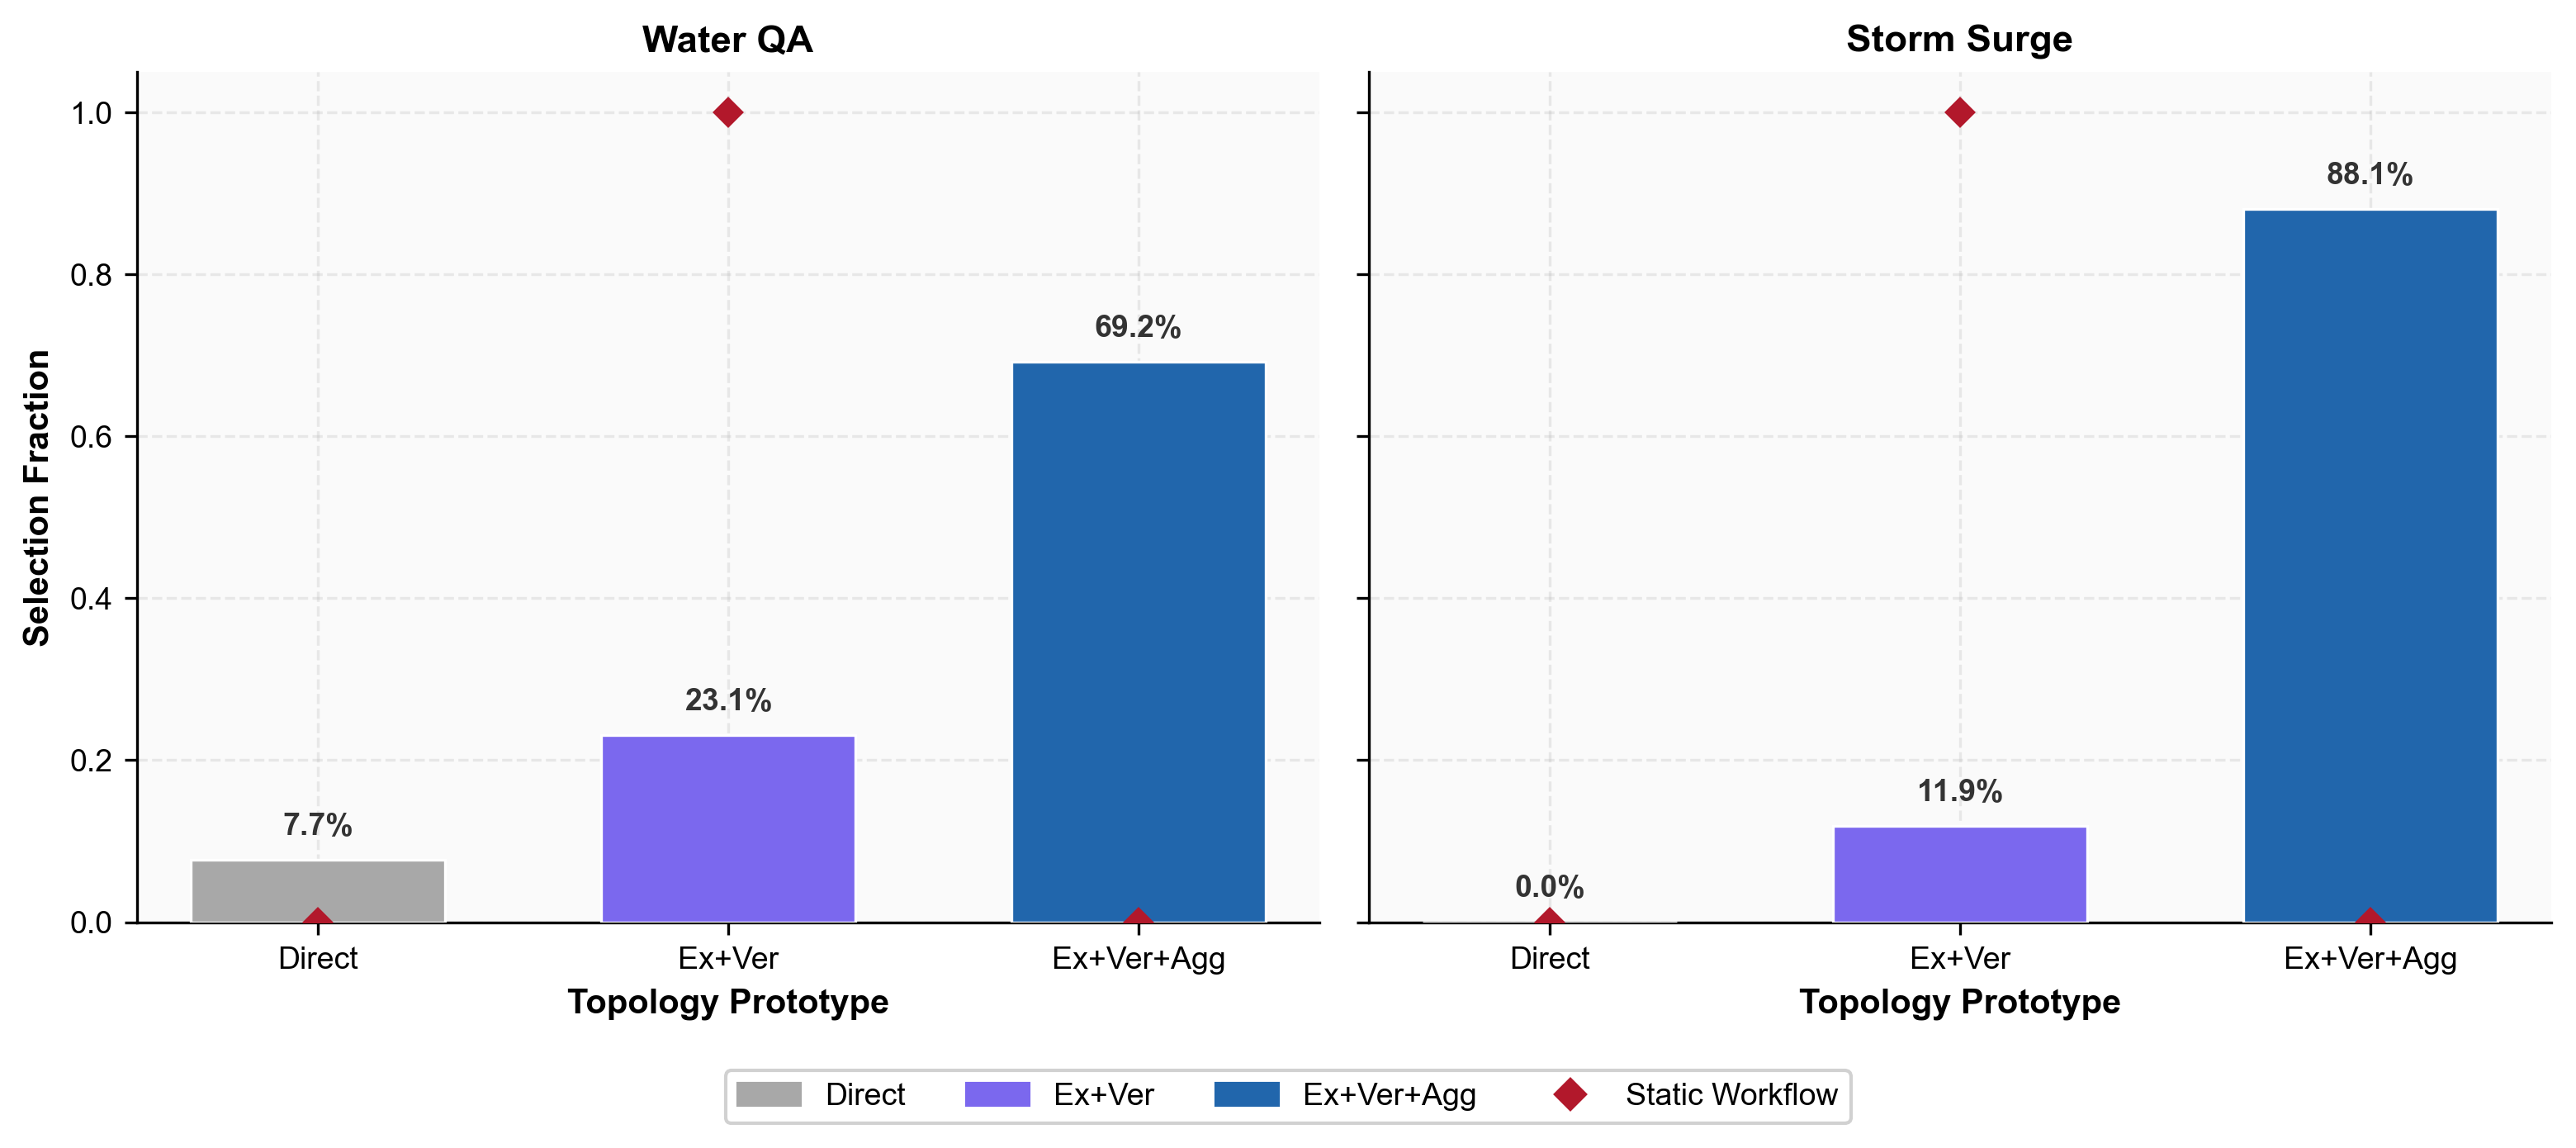
\includegraphics[width=0.96\textwidth]{figures/fig5_topology_adaptation.png}
    \Description{Two side-by-side bar charts compare selected workflow prototypes in Water QA and Storm Surge. TopoGuard uses a mixture of prototypes in Water QA and shifts toward executor-verifier-aggregator workflows in Storm Surge, while Static Workflow remains fixed.}
    \caption{Topology selection frequency across domains. TopoGuard changes its prototype choices between Water QA and Storm Surge, whereas Static Workflow remains fixed.}
    \label{fig:topo_heatmap}
\end{figure*}

\begin{table}[t]
\centering
\caption{Auxiliary transfer results on Storm Surge. The noise-perturbed contexts provide supporting evidence rather than full-scale cross-domain validation.}
\label{tab:storm_transfer}
\resizebox{0.98\linewidth}{!}{
\begin{tabular}{lcccc}
\toprule
\textbf{Method} & \textbf{Quality $S$ $\uparrow$} & \textbf{Cost ($\times 10^{-2}$ USD) $\downarrow$} & \textbf{Latency (s) $\downarrow$} & \textbf{N} \\
\midrule
TopoGuard        & 0.886           & 2.38            & 9.0  & 156 \\
Static Workflow  & 0.818           & 1.75            & 40.8 & 168 \\
Best-Quality     & \textbf{0.896} & 2.95            & 10.4 & 150 \\
Profile-Cheapest                             & 0.842           & \textbf{1.08}  & \textbf{5.7} & 144 \\
\bottomrule
\end{tabular}}
\end{table}


\subsection{Component Ablation and Repair Analysis}
\label{subsec:ablation_repair}

This section addresses \textbf{RQ2} and \textbf{RQ4}: which components drive the average performance improvement, and whether bounded local repair provides targeted recovery after intermediate execution failures.

\subparagraph{Core module ablation (Bootstrap CI + Wilcoxon).}
Table~\ref{tab:ablation_repair} summarizes the core component analysis on the 221 feasible Water QA contexts. Template and executor ablations are evaluated as paired held-out selection variants. Bounded local repair is part of the full TopoGuard execution pipeline, but its effect is failure-conditioned; therefore, the local-repair row is reported as a diagnostic pre-repair baseline from the frozen-profile recorded-execution replay rather than as a broad average main-effect comparison.

\begin{table}[t]
\centering
\caption{Core module analysis on Water QA. $\Delta S$ denotes the quality difference between the full system and each variant. Local repair is an integral execution-time component of TopoGuard, but its measured effect is failure-conditioned; the row is therefore a diagnostic baseline rather than a broad paired main-effect ablation.}
\label{tab:ablation_repair}
\resizebox{0.98\linewidth}{!}{
\begin{tabular}{lccc}
\toprule
\textbf{Variant} & \textbf{Quality $S$ $\uparrow$} & \textbf{N} & \textbf{$\Delta S$ (full $-$ ablated) $\uparrow$} \\
\midrule
TopoGuard (full)              & \textbf{0.902}          & 221       & --- \\
\quad w/o Template Selection  & 0.844          & 221 & $+0.059$ \\
\quad w/o Executor Adaptation & 0.793          & 221 & $+0.109$ \\
\quad w/o Local Repair        & 0.893          & 221 & $+0.009$ \\
\bottomrule
\end{tabular}}
\end{table}

\textbf{Analysis.} Bootstrap 95\% CI (1000 resamples, percentile method) gives $S=0.902$ [0.887, 0.918] for the full system. Template selection and executor adaptation show significant paired gains under the Wilcoxon signed-rank test. In the paired main-strategy table, the TopoGuard and w/o-Local-Repair records are tied because most contexts do not change the selected final candidate after repair gating; therefore, repair should be read through the failure-conditioned diagnostic below rather than as a broad average-performance driver.

Contribution ranking shows that executor adaptation and topology-prototype selection are the main average performance drivers. Removing \textbf{Executor Adaptation} has the largest impact ($\Delta S=+0.109$), while removing \textbf{Template Selection} yields $\Delta S=+0.059$. The local-repair diagnostic shows a smaller pre/post gap ($\Delta S=+0.009$) and is not statistically significant as a paired main effect. This does not make repair optional: it indicates that repair is not the primary source of TopoGuard's average quality gain under nominal recorded-execution replay, while remaining the execution-time recovery layer activated after detected local failures.

\subparagraph{Repair mechanism analysis (RQ4).}
In the closed-loop diagnostic, 231 of 585 monitored Water QA execution contexts trigger bounded repair (39.5\%), all activated by realized intermediate quality signals. In the corresponding no-repair condition, these triggered executions would be left unchanged after falling below the repair pass threshold. The mean gain over triggered repairs is $+0.0277$, larger than the average gain over all feasible contexts. Non-null repair actions are dominated by executor upgrades within the current topology (224 cases, 97.0\%), with smaller contributions from evaluator/verifier adjustment (5 cases, 2.2\%) and cross-topology executor repair (2 cases, 0.9\%).
\begin{table}[t]
\centering
\caption{Failure-conditioned local repair statistics on Water QA.}
\label{tab:repair_stats}
\small
\begin{tabular}{ll}
\toprule
\textbf{Statistic} & \textbf{Value} \\
\midrule
Diagnostic pre/post repair gap & $+0.009$ over feasible recorded-execution replay contexts \\
Triggered bounded repair & 231 / 585 monitored contexts \\
Repair-triggered low-quality executions left unchanged w/o repair & 231 / 585 monitored contexts \\
Mean gain per triggered repair & $+0.0277$ \\
Dominant non-null routes & Executor upgrade: 97.0\%, C2: 2.2\%, C1: 0.9\% \\
\bottomrule
\end{tabular}
\end{table}

\textbf{Complex-task local-failure stress diagnostic.}
Because the nominal recorded-execution replay contains many contexts whose initially selected workflow already exceeds the pass threshold, we additionally evaluate repair under a small set of predeclared complex execution-time failures. The profiles and initial selection policy are kept frozen; only held-out test execution is perturbed, and the diagnostic is not used to tune the profiles or the main strategy comparison. In these controlled local-failure diagnostics, bounded repair recovers more quality for local node, reasoning--computation, and verifier failures than for global evidence degradation; detailed stress results are reported in the Online Appendix.

\textbf{Simplified repair evaluation.} The replay-based repair diagnostic ranks repair candidates by frozen profile estimates before observing realized test quality, but it does not fully model all online switching overheads. Online repair execution would need to apply edit-loss to balance repair benefit against switching overhead; we leave this as future work.

Figure~\ref{fig:ablation} provides a visual summary of the stepwise contribution of executor adaptation, topology selection, and local repair.


\begin{figure*}[t]
  \centering
  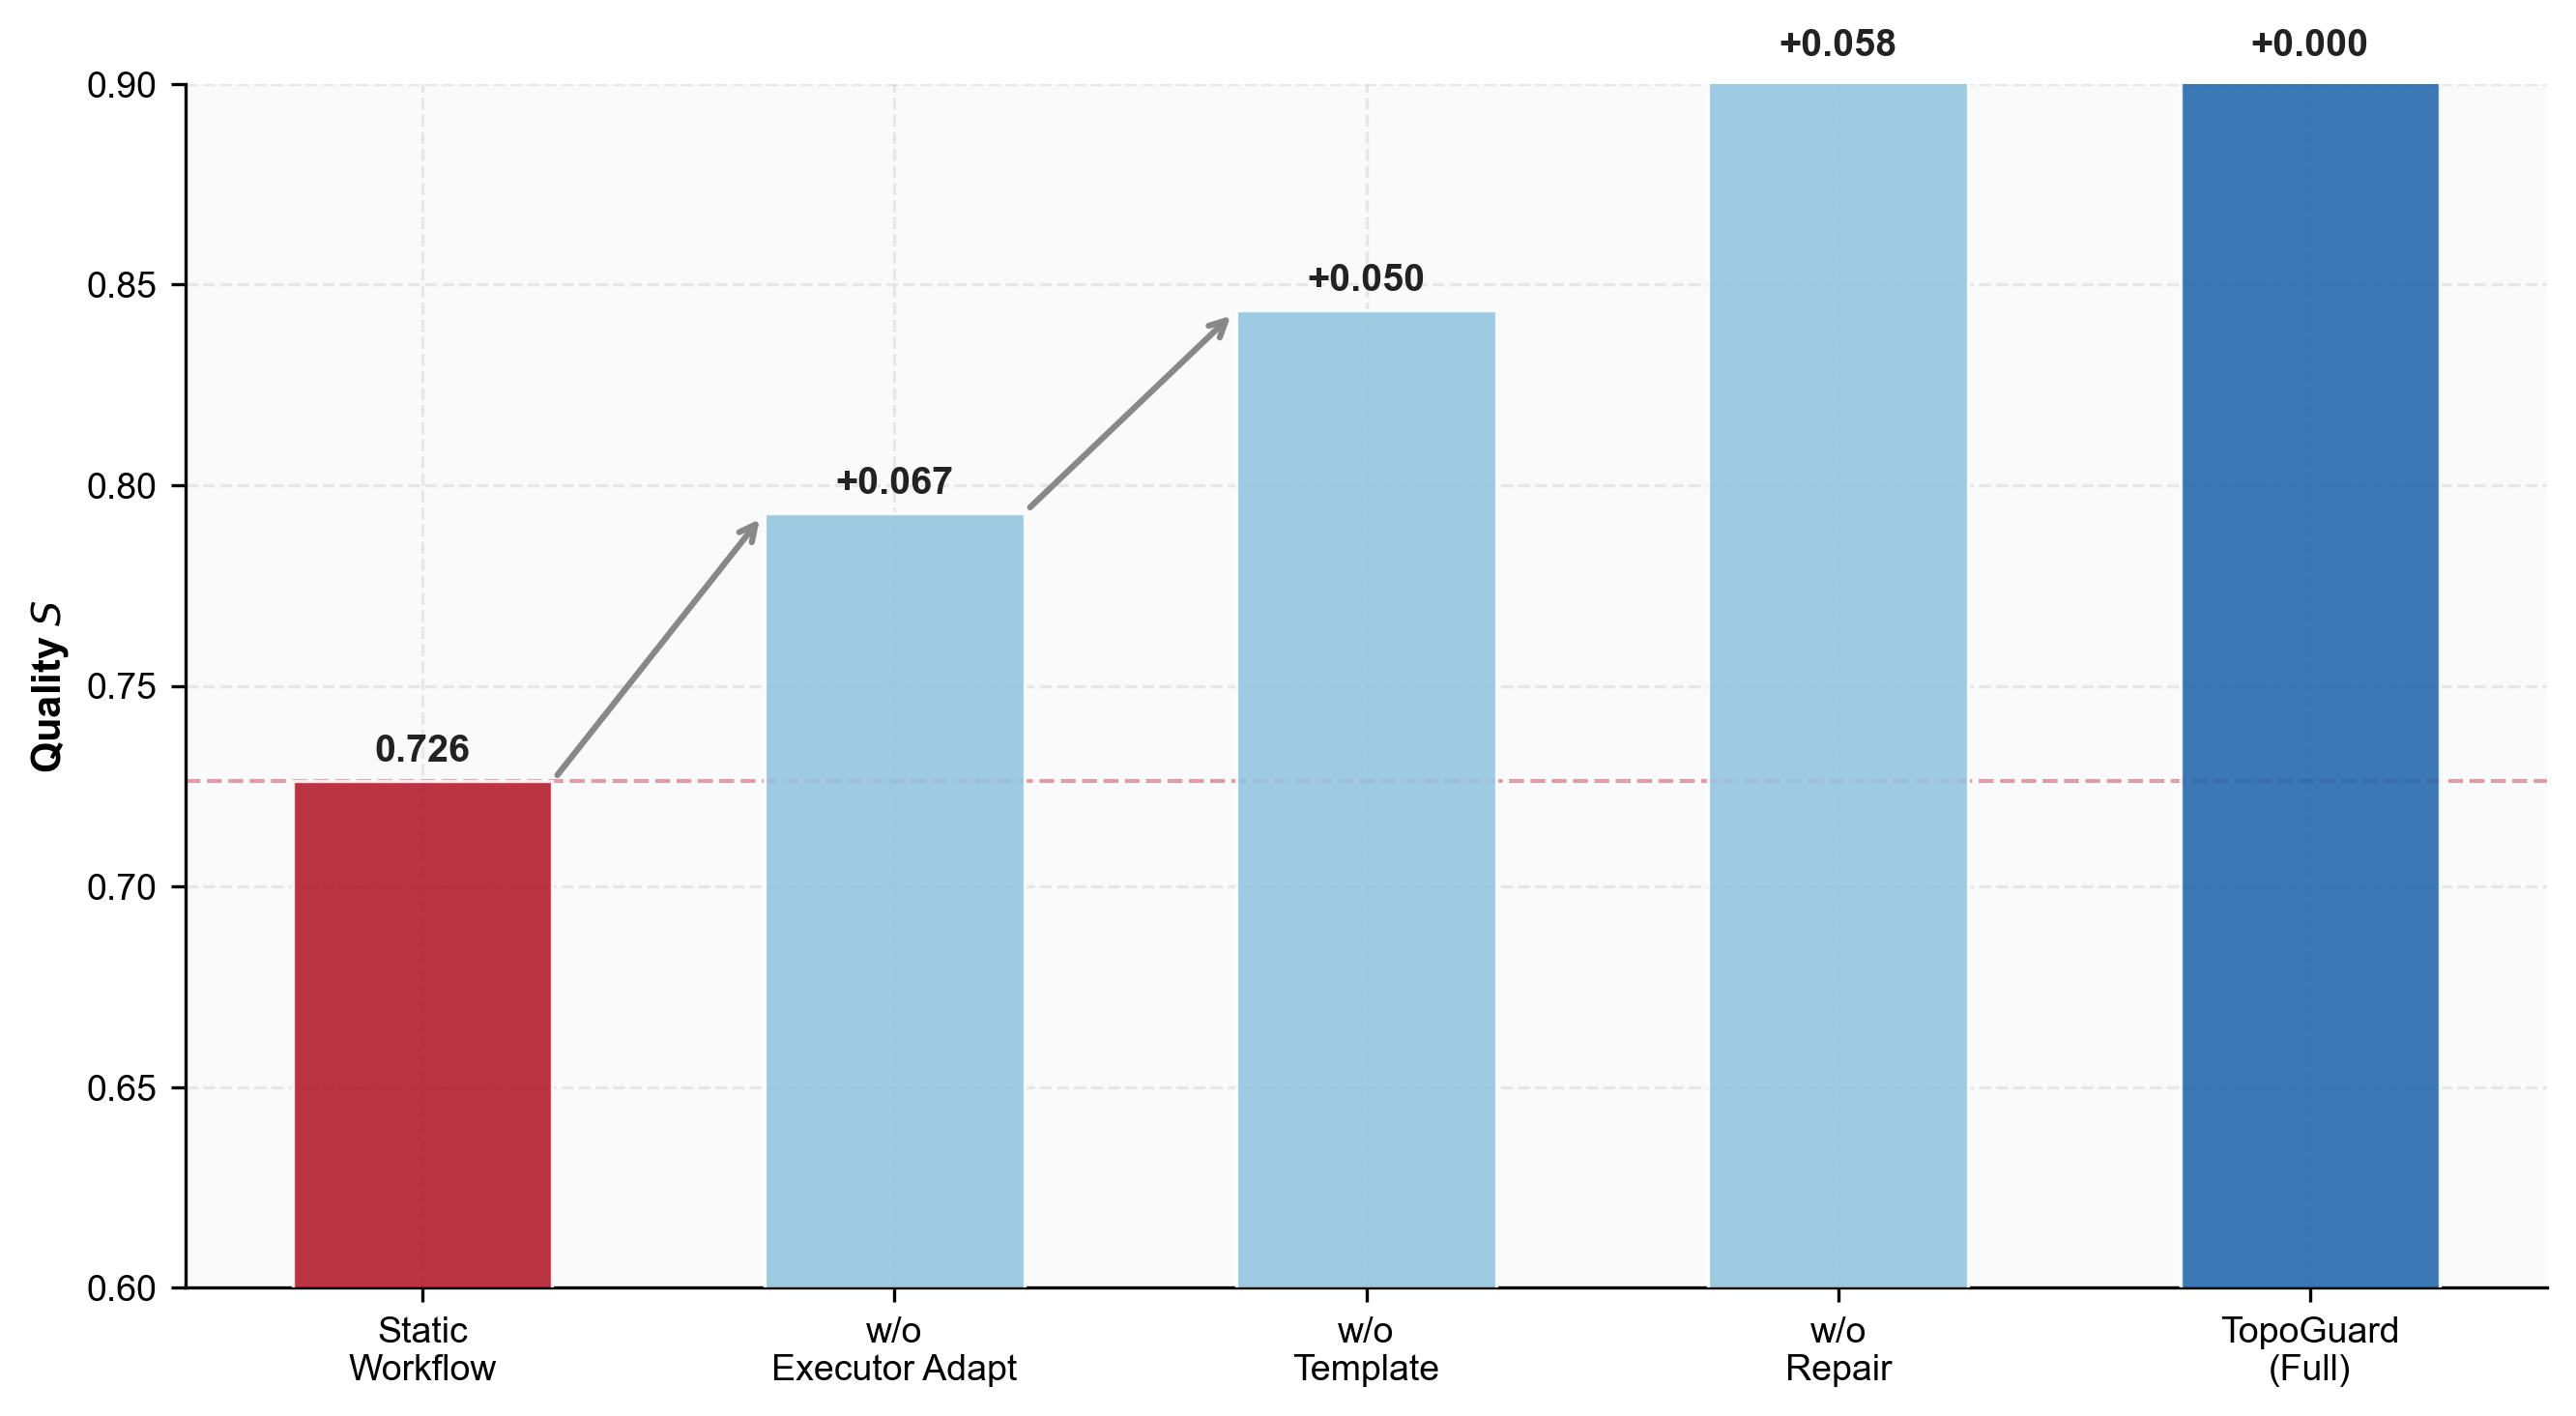
\includegraphics[width=0.98\textwidth]{figures/fig6_ablation.png}
  \Description{Bar chart showing quality scores for TopoGuard and its ablated variants sorted by quality ascending.}
  \caption{Stepwise component ablation. Executor adaptation and topology selection account for most of the average gain; local repair acts as a failure-conditioned safeguard.}
  \label{fig:ablation}
\end{figure*}

\subsection{Sensitivity to Utility Weights and Constraint Robustness}
\label{subsec:sensitivity}

We next consider \textbf{RQ3} from the perspective of utility weights and hard constraints.
A useful orchestration policy should react to changes in utility weights in a predictable way, without becoming unstable under moderate reweighting or moderate profile uncertainty \cite{cao2024online,koch2019robust}.

To test this, we vary $(\alpha,\beta,\gamma)$ and re-score candidates on the same held-out contexts without retraining the profiles.
Seven representative settings are considered, including the default configuration, quality-dominant weighting, balanced weighting, cost-priority weighting, latency-priority weighting, and two partial-objective variants. The selected workflows shift in an interpretable way as the weights change: quality-dominant weighting reaches $S=0.912$, while latency-priority weighting reduces latency at the expected cost of quality ($S=0.705$). Across all tested settings, quality remains within $S\in[0.705,0.914]$, suggesting that the method is sensitive to utility preferences but not excessively fragile. Detailed weight-sensitivity results are reported in the Online Appendix.

\textbf{Constraint-related robustness.} Because the main experiment uses hard filtering before selection, all reported strategies satisfy the estimated cost and latency constraints by construction. We therefore do not treat violation rate as a discriminative metric in the main experiment. Instead, we report feasible coverage under tightened global cost budgets and discuss profile drift as future work.

\subparagraph{Constraint stress test.}
We also evaluate how TopoGuard behaves when the normalized cost budget is varied. In this diagnostic, the same 221 of 255 contexts remain feasible across representative budget levels, and the selected average operating point remains unchanged ($S=0.902$, $C=6.402\times10^{-3}$ USD). This should be read as a sanity check rather than strong robustness evidence: under the present normalized budget scale, infeasibility is driven mainly by contexts with no viable candidate in the template library rather than by small changes around the default budget. Detailed constraint and modality-perturbation diagnostics are reported in the Online Appendix.

The aggregate results characterize the overall trade-off, but they do not show how the framework behaves within a single run. To make the execution behavior more concrete, we include a case study based on a storm-surge warning task.

\subsection{Case Study: Execution and Local Repair in a Storm-Surge Scenario}

We conduct the case study on a water-conservancy digital-twin agent platform. The platform integrates three key components: multimodal monitoring data, a task decomposition interface, and a pool of executable domain agents. This environment provides a realistic setting for evaluating how TopoGuard organizes available executors into an executable workflow for storm-surge warning tasks.

For a storm-surge warning query, the selected workflow combines textual retrieval, time-series and spatial computation, scalar verification, multimodal reasoning, and final aggregation. In the concrete execution, the default computation node underestimates uncertainty in the typhoon track forecast, producing verification scores below the pass threshold. Instead of replanning the entire workflow, TopoGuard triggers bounded local repair and replaces the computation node with a more robust variant that accounts for forecast spread while preserving reusable upstream outputs. Detailed workflow artifacts and the corresponding multimodal evidence table are provided in the Online Appendix.

The case illustrates the role of bounded local repair in high-stakes settings: the aggregate contribution of repair is small because most contexts either do not trigger repair or select the same final candidate, but the triggered-repair diagnostic shows a positive mean gain (+0.0277). In risk-sensitive domains, this targeted safeguard can reduce downstream decision failures that could propagate into incorrect warnings or missed alerts.

\subsection{Limitations and Future Work}
\label{subsec:limitations}

\textbf{Scope of multimodal modeling.} The present study addresses multimedia decision support at the workflow-structure level: different nodes consume textual, temporal, spatial, scalar, and probabilistic artifacts, and TopoGuard selects verification- or aggregation-enhanced topologies when the required modality combination or evidence reliability changes. It does not study new end-to-end fusion architectures or representation-completion models; a full missing-modality benchmark with controlled corruption of each modality is left as future work.

\textbf{Representativeness of experimental scenarios.} Both Water QA and Storm Surge come from the same water-conservancy digital-twin platform with relatively limited sample sizes. The Storm Surge auxiliary transfer experiment covers fewer (node type, difficulty) combinations than Water QA, constituting small-sample supporting evidence rather than full-scale validation. Generalization claims across domains require verification in more diverse real-world settings.

\textbf{Hard-constraint stress testing.} The main experiment enforces ex-ante estimated feasibility by pre-filtering candidates against budget and latency constraints. This design isolates the effect of selection heuristics under the same feasible candidate space, but it does not fully characterize behavior when the feasible set becomes sparse or empty. The constraint stress test in Table~\ref{tab:constraint_stress} partially addresses this issue by tightening the cost budget and reporting feasible coverage; more extensive stress tests with larger template libraries, cold-start profiles, and explicit empty-set recovery policies remain future work.

\textbf{External validity of the recorded-execution replay protocol.} All main results are based on a frozen-profile recorded-execution replay protocol using historical profile lookups, not a live online deployment. This protocol does not account for executor performance drift over time or cold-start scenarios where new tasks lack historical profiles. A more realistic dynamic profile update mechanism (e.g., online Bayesian updates in the profile manager) has not been validated end-to-end.

\textbf{Representativeness of the static baseline.} The Static Workflow configuration (executor+verifier + Kimi-K2.5 executor) is a representative fixed-topology choice under the experimental budget constraints, not a hand-optimized strongest static topology. The equal-budget fixed-topology analysis provides an initial check against stronger fixed alternatives, but a broader suite of hand-designed fixed workflows and domain-specific pipelines would further strengthen external validity.

\textbf{Proxy comparison with workflow generation methods.} We include an AFlow-Style Offline Search baseline instantiated within the same auditable topology space, but this is not a full reproduction of AFlow, AutoFlow, or WorkflowLLM. Full workflow-generation systems target unconstrained offline structure optimization on different benchmarks such as code generation and planning. Directly adapting them to our hard cost--latency constraints and multimodal decision setting remains future work.

\textbf{Empirically set edit-loss weights.} The edit-loss weights $\lambda_n=0.30$, $\lambda_\phi=0.25$, etc.\ are set from engineering experience and have not been systematically optimized. Sensitivity analysis for $\tau_{\mathrm{pass}}$ and systematic experiments for the edit-loss weights remain as future work.

These limitations delimit the scope of the present results and point to important directions for future validation.

\subsection{Discussion}
\label{subsec:discussion}

TopoGuard improves quality relative to a fixed static workflow ($S=0.902$ vs.\ $0.726$, $\Delta S=+0.176$), while staying close to the quality-maximizing baseline on Water QA ($0.902$ vs.\ $0.914$) and within 1.1 percentage points of Best-Quality on Storm Surge. The experiments show that TopoGuard mainly improves the quality side of the feasible quality--cost--latency trade-off, while avoiding the high-latency Best-Quality operating point.

The cost-adjusted paired regression shows a positive intercept ($\beta_0=+0.1266$), suggesting that TopoGuard's quality advantage includes a component not explained by cost increase alone. The ablation results more directly show that executor adaptation and topology-prototype selection account for most of the average gain. TopoGuard achieves $S=0.920$ on easy, $S=0.915$ on medium, and $S=0.851$ on hard contexts, with an overall advantage of $\Delta S=+0.176$ over the static baseline ($S=0.726$). Bounded local repair is the execution-time adaptation layer of TopoGuard. It is not a significant paired main-effect driver under nominal recorded-execution replay, but it provides a mean gain of $+0.0277$ when triggered and larger recovery in a small controlled local-failure diagnostic. Executor upgrade within the current topology is the dominant repair route. Bounded local repair is therefore best interpreted as a targeted execution-time safeguard rather than the primary average performance driver.

\section{Conclusion}
\label{sec:conclusion}

This paper presented TopoGuard, a profile-guided adaptive topology orchestration framework for risk-sensitive multimodal decision support. TopoGuard maintains quality--cost--latency profiles for candidate auditable workflow DAG prototypes and executor assignments, selects an initial feasible topology through constrained Pareto pruning, and applies bounded local repair when intermediate execution quality degrades. A trace-based evaluation with frozen profiles over execution records from a water-conservancy digital-twin platform shows that TopoGuard stays close to the quality-maximizing baseline on Water QA ($S=0.902$ vs.\ $0.914$) while reducing latency (77.6\,s vs.\ 118.9\,s), and improves over fixed workflows, executor-only routing, and offline-search proxy baselines in the feasible replay comparison. The component, difficulty-wise, and repair analyses suggest that the full TopoGuard system improves over the static baseline by $\Delta S=+0.176$. Executor adaptation and topology-prototype selection are the main average performance drivers, while bounded local repair serves as the failure-conditioned execution-time adaptation layer: it is not significant as a paired main effect under nominal recorded-execution replay, but it yields a mean gain when triggered ($+0.0277$) and larger recovery in a small controlled local-failure diagnostic.


\clearpage
\newpage
\bibliographystyle{ACM-Reference-Format}
\bibliography{reference}

\clearpage
\appendix
\section*{Online Appendix}
\label{sec:online_appendix}

\subsection*{A. Additional Pareto-Frontier Visualization}

Figure~\ref{fig:pareto_frontier} shows the feasible quality--cost and quality--latency spaces for the Water QA candidate pool. This visualization is auxiliary to the main Water QA comparison in Table~\ref{tab:water_qa_main}; it illustrates the trade-off geometry but does not define an additional evaluation metric.

\begin{figure*}[h]
    \centering
    
\includegraphics[width=0.96\textwidth]{figures/fig4_pareto_frontier.png}
    \Description{Left: Pareto frontier in quality-cost space with step frontier and candidate points. Right: Pareto frontier in quality-latency space.}
    \caption{Auxiliary Pareto-frontier visualization of the feasible Water QA candidate space. Left: quality--cost trade-off. Right: quality--latency trade-off. Strategy markers show average operating points.}
    \label{fig:pareto_frontier}
\end{figure*}

\subsection*{B. Complex Local-Failure Stress Diagnostic}

For the complex-task repair diagnostic, profiles and the initial selection policy are kept frozen; only held-out test execution is perturbed. Local-failure scenarios degrade the selected node output as a controlled proxy for an executor or intermediate multimodal artifact failing on a complex instance, while repair candidates are selected from the same profile library before their realized quality is observed. Table~\ref{tab:complex_repair_stress} reports the detailed stress results.

\begin{table}[h]
\centering
\caption{Complex-task local-failure stress diagnostic for TopoGuard. $n$ denotes predeclared stress context groups; $S_{\mathrm{shock}}$ is the quality after test-time degradation before repair.}
\label{tab:complex_repair_stress}
\begin{tabular}{lccccc}
\toprule
Stress scenario & $n$ & $S_{\mathrm{nominal}}$ & $S_{\mathrm{shock}}$ & $S_{\mathrm{repair}}$ & $\Delta S$ \\
\midrule
Hard local node failure & 3 & 0.854 & 0.495 & 0.606 & +0.110 \\
Hard reasoning--computation failure & 3 & 0.854 & 0.470 & 0.732 & +0.263 \\
Medium--hard verifier failure & 3 & 0.787 & 0.456 & 0.622 & +0.166 \\
Hard global evidence degradation & 3 & 0.854 & 0.641 & 0.661 & +0.021 \\
\bottomrule
\end{tabular}
\end{table}

The diagnostic clarifies the operational boundary of repair. When the failure is local to a node or executor, bounded repair recovers part of the lost quality without global replanning. When the degradation is global to the evidence stream, the improvement is much smaller because replacement candidates face the same degraded evidence.

\subsection*{C. Utility, Constraint, and Perturbation Diagnostics}

Table~\ref{tab:sensitivity_simple} reports the utility-weight sensitivity analysis. The selected workflows shift in an interpretable way as the weights change, and the quality range remains bounded across the tested settings.

\begin{table}[h]
\centering
\caption{Sensitivity analysis under different utility weight settings.}
\label{tab:sensitivity_simple}
\small
\begin{tabular}{lcccc}
\toprule
\textbf{Weight Setting} & $\alpha$ & $\beta$ & $\gamma$ & \textbf{$S$ $\uparrow$} \\
\midrule
Default (quality-centric) & 0.65 & 0.25 & 0.10 & 0.902 \\
Quality-dominant         & 0.92 & 0.05 & 0.03 & 0.912 \\
Balanced                 & 0.50 & 0.30 & 0.20 & 0.824 \\
Cost-priority             & 0.40 & 0.50 & 0.10 & 0.853 \\
Latency-priority          & 0.10 & 0.10 & 0.80 & 0.705 \\
Q+C only                  & 0.80 & 0.20 & 0.00 & \textbf{0.914} \\
Q+L only                  & 0.80 & 0.00 & 0.20 & 0.853 \\
\bottomrule
\end{tabular}
\end{table}

\begin{table}[h]
\centering
\caption{Constraint stress test under tightened cost budgets. Quality is computed only over remaining feasible contexts.}
\label{tab:constraint_stress}
\small
\begin{tabular}{lcccc}
\toprule
\textbf{Budget Level} & \textbf{Feasible\%} & \textbf{$S$ $\uparrow$} & \textbf{$C$ ($\times 10^{-3}$ USD) $\downarrow$} & \textbf{Topology Shift} \\
\midrule
C$_{\max}=0.30$ & 86.7\% & 0.902 & 6.402 & stable \\
C$_{\max}=0.50$ & 86.7\% & 0.902 & 6.402 & stable \\
C$_{\max}=0.70$ & 86.7\% & 0.902 & 6.402 & stable \\
\bottomrule
\end{tabular}
\end{table}

As a controlled evidence-degradation diagnostic, we reduce quality estimates for specific modality-consuming node types. Removing spatial, textual, or scalar evidence causes 17 topology shifts in the affected settings, while the noisy-sensor perturbation leaves the selected topology distribution unchanged. This diagnostic suggests that topology selection can respond to modality-specific profile changes, but more realistic perturbations where relative rankings within a node type change are needed to fully evaluate multimodal uncertainty adaptation.

\end{document}

